 
%%% DOCUMENTCLASS 
%%%-------------------------------------------------------------------------------

\documentclass[
a4paper, % Stock and paper size.
10pt, % Type size.
% article,
% oneside, 
onecolumn, % Only one column of text on a page.
% openright, % Each chapter will start on a recto page.
% openleft, % Each chapter will start on a verso page.
openany, % A chapter may start on either a recto or verso page.
]{memoir}

%%% PACKAGES 
%%%------------------------------------------------------------------------------

\usepackage[utf8x]{inputenc} % If utf8 encoding
% \usepackage[lantin1]{inputenc} % If not utf8 encoding, then this is probably the way to go
\usepackage[T1]{fontenc}    %
\usepackage[english]{babel} % English please
\usepackage[final]{microtype} % Less badboxes

% \usepackage{kpfonts} %Font

\usepackage{amsmath,amssymb,mathtools} % Math

% \usepackage{tikz} % Figures
\usepackage{graphicx} % Include figures

\usepackage{listings}    % Add code snippets
\usepackage[usenames,dvipsnames,svgnames,table]{xcolor}

\usepackage[linktocpage=true]{hyperref} % Extensive support for hypertext in LaTeX
\usepackage[usenames,dvipsnames]{xcolor} %used for font color
\usepackage{dirtree} % Make directory trees easily
\usepackage{framed} % shade in a region of the page
\usepackage{multirow}  % use rows spanning multiple columns in tables
\usepackage{float}
\usepackage[all]{background}
\usepackage[hyphenbreaks]{breakurl}
\usepackage{tcolorbox}
%%% PAGE LAYOUT 
%%%------------------------------------------------------------------------------

\setlrmarginsandblock{0.15\paperwidth}{*}{1} % Left and right margin
\setulmarginsandblock{0.2\paperwidth}{*}{1}  % Upper and lower margin
\checkandfixthelayout

%%% SECTIONAL DIVISIONS
%%%------------------------------------------------------------------------------

\maxsecnumdepth{subsubsection} % Subsections (and higher) are numbered
\setsecnumdepth{subsubsection}

\makeatletter %
\makechapterstyle{standard}{
  \setlength{\beforechapskip}{0\baselineskip}
  \setlength{\midchapskip}{1\baselineskip}
  \setlength{\afterchapskip}{2\baselineskip}
  \renewcommand{\chapterheadstart}{\vspace*{\beforechapskip}}
  \renewcommand{\chapnamefont}{\centering\normalfont\huge}
  \renewcommand{\printchaptername}{\chapnamefont \@chapapp}
  \renewcommand{\chapternamenum}{\space}
  \renewcommand{\chapnumfont}{\normalfont\huge}
  \renewcommand{\printchapternum}{\chapnumfont \thechapter}
  \renewcommand{\afterchapternum}{\par\nobreak\vskip \midchapskip}
  \renewcommand{\printchapternonum}{\vspace*{\midchapskip}\vspace*{5mm}}
  \renewcommand{\chaptitlefont}{\centering\bfseries\HUGE}
  \renewcommand{\printchaptertitle}[1]{\chaptitlefont ##1}
  \renewcommand{\afterchaptertitle}{\par\nobreak\vskip \afterchapskip}
}
\makeatother

\chapterstyle{standard}

\setsecheadstyle{\normalfont\huge\bfseries}
\setsubsecheadstyle{\normalfont\large\bfseries}
\setparaheadstyle{\normalfont\normalsize\bfseries}
\setparaindent{0pt}\setafterparaskip{0pt}

%%% FLOATS AND CAPTIONS
%%%------------------------------------------------------------------------------

\makeatletter                  % You do not need to write [htpb] all the time
\renewcommand\fps@figure{htbp} %
\renewcommand\fps@table{htbp}  %
\makeatother                   %

\captiondelim{\space } % A space between caption name and text
\captionnamefont{\small\bfseries} % Font of the caption name
\captiontitlefont{\small\normalfont} % Font of the caption text

\changecaptionwidth          % Change the width of the caption
\captionwidth{1\textwidth} %

%%% ABSTRACT
%%%------------------------------------------------------------------------------

\renewcommand{\abstractnamefont}{\normalfont\small\bfseries} % Font of abstract title
\setlength{\absleftindent}{0.1\textwidth} % Width of abstract
\setlength{\absrightindent}{\absleftindent}

%%% HEADER AND FOOTER 
%%%------------------------------------------------------------------------------

\makepagestyle{standard} % Make standard pagestyle

\makeatletter                 % Define standard pagestyle
\makeevenfoot{standard}{}{}{} %
\makeoddfoot{standard}{}{}{}  %
\makeevenhead{standard}{\bfseries\thepage\normalfont\qquad\small\leftmark}{}{}
\makeoddhead{standard}{}{}{\small\rightmark\qquad\bfseries\thepage}
% \makeheadrule{standard}{\textwidth}{\normalrulethickness}
\makeatother                  %

\makeatletter
\makepsmarks{standard}{
\createmark{chapter}{both}{shownumber}{\@chapapp\ }{ \quad }
\createmark{section}{right}{shownumber}{}{ \quad }
\createplainmark{toc}{both}{\contentsname}
\createplainmark{lof}{both}{\listfigurename}
\createplainmark{lot}{both}{\listtablename}
\createplainmark{bib}{both}{\bibname}
\createplainmark{index}{both}{\indexname}
\createplainmark{glossary}{both}{\glossaryname}
}
\makeatother                               %

\makepagestyle{chap} % Make new chapter pagestyle

\makeatletter
\makeevenfoot{chap}{}{\small\bfseries\thepage}{} % Define new chapter pagestyle
\makeoddfoot{chap}{}{\small\bfseries\thepage}{}  %
\makeevenhead{chap}{}{}{}   %
\makeoddhead{chap}{}{}{}    %
% \makeheadrule{chap}{\textwidth}{\normalrulethickness}
\makeatother

\nouppercaseheads
\pagestyle{standard}               % Choosing pagestyle and chapter pagestyle
\aliaspagestyle{chapter}{chap} %

%%% NEW COMMANDS
%%%------------------------------------------------------------------------------
% custom commands defined in here (must be called before constants)
%%%%%%%%%%%%%%%%%%%%%%%%%%%%%%%%%%%%%%%%%%%%%%%%%%%%%%%%
%%
%%  New colours
%%
%%%%%%%%%%%%%%%%%%%%%%%%%%%%%%%%%%%%%%%%%%%%%%%%%%%%%%%%

\definecolor{codegreen}{rgb}{0,0.6,0}
\definecolor{codegray}{rgb}{0.5,0.5,0.5}
\definecolor{codepurple}{rgb}{0.58,0,0.82}
\definecolor{darkgray}{rgb}{0.20,0.20,0.20}
\definecolor{backcolour1}{rgb}{0.95,0.95,0.92}
\definecolor{backcolour2}{rgb}{1,0.977,0.801}
\definecolor{backcolour3}{rgb}{0.79,0.88,1}


%%%%%%%%%%%%%%%%%%%%%%%%%%%%%%%%%%%%%%%%%%%%%%%%%%%%%%%%
%%
%%  formatting constants
%%
%%%%%%%%%%%%%%%%%%%%%%%%%%%%%%%%%%%%%%%%%%%%%%%%%%%%%%%%

% formatting the named variables (from user setup)
\newcommand{\definevariable}[1]{\textcolor{blue}{\{#1\}}}
\newcommand{\definevariablecmd}[1]{\textcolor{cyan}{\{#1\}}}

% --------------------------------------------------------
% formatting the named keywords 
\newcommand{\definekeyword}[1]{\textcolor{red}{\{#1\}}}

% --------------------------------------------------------
% Program should be in small caps
\newcommand{\Program}[1]{\textsc{#1}}

% --------------------------------------------------------
% Double underscore
\newlength\dunder
\settowidth{\dunder}{\_}
\newcommand{\twound}{\rule{1.25\dunder}{0.2pt}}

% --------------------------------------------------------
% formatting for the directories trees
\newcommand{\customdirtree}[1]{
\renewcommand*\DTstylecomment{\ttfamily\textcolor{black}}
\renewcommand*\DTstyle{\ttfamily\textcolor{blue}}
\dirtree{%
#1}
}

% --------------------------------------------------------
% Parameters
% \ParameterEntry{Name}{Description}{variable}{default value}{used in}{location}{level (if dev)}
\newcommand{\ParameterEntry}[8]{
	\begin{minipage}[t]{\textwidth}
	\textbf{#1 (\textcolor{red}{#3})}

	\begin{thighlight}
	\textcolor{brown}{#2} 

	\begin{tabular}{>{\color{red}}l c l}
	&&\\
	#3 & = & #4 \\
	&&\\
	\textcolor{blue}{Used in:}  & \multicolumn{2}{p{10cm}}{#5} \\
	\textcolor{blue}{Defined in:} & \multicolumn{2}{p{10cm}}{#6} \\
	\ifdevguide
	\textcolor{blue}{Called in:} & \multicolumn{2}{p{10cm}}{\textcolor{codegreen}{#7}} \\
	\textcolor{blue}{Level:} & \multicolumn{2}{p{10cm}}{#8} \\
	\fi
	\end{tabular}
	\end{thighlight}
	\end{minipage}
}


\newcommand{\PseudoParamEntry}[7]{
	\begin{minipage}[t]{\textwidth}
	\textbf{#1 (\textcolor{red}{#3})}

	\begin{thighlight}
	\textcolor{codegreen}{#2} 

	\begin{tabular}{>{\color{red}}l c l}
	&&\\
	#3 && \\
	&&\\
	\textcolor{blue}{Used in:}  & \multicolumn{2}{p{10cm}}{#4} \\
	\textcolor{blue}{Defined in:} & \multicolumn{2}{p{10cm}}{#5} \\
	\ifdevguide
	\textcolor{blue}{Called in:} & \multicolumn{2}{p{10cm}}{\textcolor{codegreen}{#6}} \\
	\textcolor{blue}{Level:} & \multicolumn{2}{p{10cm}}{#7} \\
	\fi
	\end{tabular}
	\end{thighlight}
	\end{minipage}
}


% --------------------------------------------------------
% define dev sections notes etc

\newcommand{\devsection}[2]{
\ifdevguide
\section{#1}

#2
\fi
}


\newcommand{\DevNote}[1]{
\ifdevguide
\begin{note}
#1
\end{note}
\fi
}
% get code highlighting parameters

\lstdefinestyle{text}{
    commentstyle=\color{codegreen},
    keywordstyle=\color{magenta},
    numberstyle=\tiny\color{codegray},
    stringstyle=\color{codepurple},
    basicstyle=\linespread{1.2}\ttfamily\footnotesize,
    breakatwhitespace=false,         
    breaklines=true,                 
    captionpos=b,                    
    keepspaces=true,                 
    % numbers=left,                    
    % numbersep=5pt,                  
    showspaces=false,                
    showstringspaces=false,
    showtabs=false,                  
    tabsize=2,
    moredelim=**[is][\color{red}]{@}{@},
    moredelim=**[is][\color{OliveGreen}]{<}{>},
    extendedchars=false,
    columns=fullflexible,
    escapeinside={(*}{*)},%
	  literate={\\@}{{\unichar{"0040}}}1
			 {\\<}{{\unichar{"003C}}}1 
			 {\\>}{{\unichar{"003E}}}1
}

\lstdefinestyle{bashstyle}{
	language=bash,  
    commentstyle=\color{codegreen},
    keywordstyle=\color{magenta},
    numberstyle=\tiny\color{codegray},
    stringstyle=\color{codepurple},
    basicstyle=\linespread{1.2}\ttfamily\footnotesize,
    breakatwhitespace=false,         
    breaklines=true,                 
    captionpos=b,                    
    keepspaces=true,                 
    % numbers=left,                    
    % numbersep=5pt,                  
    showspaces=false,                
    showstringspaces=false,
    showtabs=false,                  
    tabsize=2,
    moredelim=**[is][\color{red}]{@}{@},
    moredelim=**[is][\color{OliveGreen}]{<}{>},
    extendedchars=false,
    columns=fullflexible,
    escapeinside={(*}{*)},%
    literate={\\@}{{\unichar{"0040}}}1
       {\\<}{{\unichar{"003C}}}1 
       {\\>}{{\unichar{"003E}}}1
}


\lstdefinestyle{cshstyle}{
  language=sh,  
    commentstyle=\color{codegreen},
    keywordstyle=\color{magenta},
    numberstyle=\tiny\color{codegray},
    stringstyle=\color{codepurple},
    basicstyle=\linespread{1.2}\ttfamily\footnotesize,
    breakatwhitespace=false,         
    breaklines=true,                 
    captionpos=b,                    
    keepspaces=true,                 
    % numbers=left,                    
    % numbersep=5pt,                  
    showspaces=false,                
    showstringspaces=false,
    showtabs=false,                  
    tabsize=2,
    moredelim=**[is][\color{red}]{@}{@},
    moredelim=**[is][\color{OliveGreen}]{<}{>},
    extendedchars=false,
    columns=fullflexible,
    escapeinside={(*}{*)},%
    literate={\\@}{{\unichar{"0040}}}1
       {\\<}{{\unichar{"003C}}}1 
       {\\>}{{\unichar{"003E}}}1
}

\lstdefinestyle{cmdstyle}{
    language=command.com,
    commentstyle=\color{codegreen},
    keywordstyle=\color{blue!35!white},
    numberstyle=\tiny\color{codegray},
    stringstyle=\color{codepurple},
    basicstyle=\linespread{1.2}\ttfamily\footnotesize\color{white},
    breakatwhitespace=false,         
    breaklines=true,                 
    captionpos=b,                    
    keepspaces=true,                 
    % numbers=left,                    
    % numbersep=5pt,                  
    showspaces=false,                
    showstringspaces=false,
    showtabs=false,                  
    tabsize=2,
    extendedchars=false,
    columns=fullflexible,
    morekeywords={chmod, unzip},
    escapeinside={(*}{*)},%
}

\lstdefinestyle{cmdstyleprint}{
    commentstyle=\color{codegreen},
    keywordstyle=\color{blue!35!white},
    numberstyle=\tiny\color{codegray},
    stringstyle=\color{codepurple},
    basicstyle=\linespread{1.2}\ttfamily\footnotesize\color{white},
    breakatwhitespace=false,         
    breaklines=true,                 
    captionpos=b,                    
    keepspaces=true,                 
    % numbers=left,                    
    % numbersep=5pt,                  
    showspaces=false,                
    showstringspaces=false,
    showtabs=false,                  
    tabsize=2,
    extendedchars=false,
    columns=fullflexible,
    morekeywords={chmod, unzip},
    escapeinside={(*}{*)},%
}

\lstdefinestyle{pythonstyle}{
    language=Python,
    commentstyle=\color{codegreen},
    keywordstyle=\color{magenta},
    numberstyle=\tiny\color{codegray},
    stringstyle=\color{codepurple},
    basicstyle=\linespread{1.2}\ttfamily\footnotesize,
    breakatwhitespace=false,         
    breaklines=true,                 
    captionpos=b,                    
    keepspaces=true,                 
    % numbers=left,                    
    % numbersep=5pt,                  
    showspaces=false,                
    showstringspaces=false,
    showtabs=false,                  
    tabsize=2,
    moredelim=**[is][\color{red}]{@}{@},
    extendedchars=false,
    columns=fullflexible,
    escapeinside={(*}{*)},%
    literate={\\@}{{\unichar{"0040}}}1
}


\lstdefinestyle{pythoninline}{
    language=Python,
    backgroundcolor=\color{backcolour3},   
    commentstyle=\color{codegreen},
    keywordstyle=\color{magenta},
    numberstyle=\tiny\color{codegray},
    stringstyle=\color{codepurple},
    basicstyle=\ttfamily\scriptsize,
    breakatwhitespace=false,         
    breaklines=true,                 
    captionpos=b,                    
    keepspaces=true,                 
    % numbers=left,                    
    % numbersep=5pt,                  
    showspaces=false,                
    showstringspaces=false,
    showtabs=false,                  
    tabsize=2,
    moredelim=**[is][\color{red}]{@}{@},
    extendedchars=false,
    columns=fullflexible,
    literate={\\@}{{\unichar{"0040}}}1
}

\tcbuselibrary{listings}
\tcbuselibrary{breakable}

% example:
% \newtcblisting{mylisting}{
%       arc=0pt,
%       top=0mm,
%       bottom=0mm,
%       left=0mm,
%       right=0mm,
%       boxrule=0pt,
%       colback=black,
%       listing only,
%       listing options={style=mystyle},
%       hbox
% }


\newtcblisting{textbox}{
      before skip=3pt,
      after skip=6pt,
      %tcbox raise base,
      top=0pt,bottom=0pt,left=0mm,right=0mm,
      %toprule=0.3mm,bottomrule=0.3mm,boxsep=0.5mm,
      colback=backcolour1,
      colframe=backcolour1!75!black,
      fonttitle={\tiny\bfseries},
      title={text},  % Fixed title
      listing only,
      listing options={style=text},
}

\newtcblisting{bashbox}{
      before skip=3pt,
      after skip=6pt,
      %tcbox raise base,
      top=0pt,bottom=0pt,left=2mm,right=0mm,
      %toprule=0.3mm,bottomrule=0.3mm,boxsep=0.5mm,
      colback=backcolour1,
      colframe=backcolour1!75!black,
      fonttitle={\tiny\bfseries},
      title={bash},  % Fixed title
      listing only,
      listing options={style=bashstyle},
}

\newtcblisting{cshbox}{
      before skip=3pt,
      after skip=6pt,
      %tcbox raise base,
      top=0pt,bottom=0pt,left=0mm,right=0mm,
      %toprule=0.3mm,bottomrule=0.3mm,boxsep=0.5mm,
      colback=backcolour1,
      colframe=backcolour1!75!black,
      fonttitle={\tiny\bfseries},
      title={tcsh/csh},  % Fixed title
      listing only,
      listing options={style=cshstyle},
}

\newtcblisting{cmdbox}{
      before skip=3pt,
      after skip=6pt,
      %tcbox raise base,
      top=0pt,bottom=0pt,left=2mm,right=0mm,
      %toprule=0.3mm,bottomrule=0.3mm,boxsep=0.5mm,
      colback=darkgray,
      colframe=darkgray!75!black,
      fonttitle={\tiny\bfseries},
      title={CMD input},  % Fixed title
      listing only,
      listing options={style=cmdstyle},
      every listing line={\textcolor{red}{\small\ttfamily\bfseries \textgreater{\textgreater}\,\,\,}}
}

\newtcblisting{cmdboxprint}{
      before skip=3pt,
      after skip=6pt,
      %tcbox raise base,
      top=0pt,bottom=0pt,left=2mm,right=0mm,
      %toprule=0.3mm,bottomrule=0.3mm,boxsep=0.5mm,
      colback=darkgray,
      colframe=darkgray!75!black,
      fonttitle={\tiny\bfseries},
      title={Command line output},  % Fixed title
      listing only,
      listing options={style=cmdstyleprint}
}

\newtcblisting{pythonbox}{
      before skip=3pt,
      after skip=6pt,
      %tcbox raise base,
      top=0pt,bottom=0pt,left=2mm,right=0mm,
      %toprule=0.3mm,bottomrule=0.3mm,boxsep=0.5mm,
      colback=backcolour3,
      colframe=backcolour3!75!black,
      fonttitle={\tiny\bfseries},
      title={Python/Ipython},  % Fixed title
      listing only,
      listing options={style=pythonstyle},
}

\newtcolorbox{note}[1][]{%
  enhanced jigsaw, % better frame drawing
  borderline west={2pt}{0pt}{red}, % straigh vertical line at the left edge
  sharp corners, % No rounded corners
  boxrule=0pt, % no real frame,
  fonttitle={\large\bfseries},
  coltitle={black},  % Black colour for title
  title={Note:\ },  % Fixed title
  attach title to upper, % Move the title into the box
  #1
}

\newtcolorbox{todo}[1][]{%
  enhanced jigsaw, % better frame drawing
  borderline west={2pt}{0pt}{green}, % straigh vertical line at the left edge
  sharp corners, % No rounded corners
  boxrule=0pt, % no real frame,
  fonttitle={\large\bfseries},
  coltitle={black},  % Black colour for title
  title={TODO:\ },  % Fixed title
  attach title to upper, % Move the title into the box
  #1
}


\newtcolorbox{thighlight}[1][]{%
  enhanced jigsaw, % better frame drawing
  before skip=3pt,
  after skip=6pt,
  borderline west={2pt}{0pt}{orange}, % straigh vertical line at the left edge
  sharp corners, % No rounded corners
  boxrule=0pt, % no real frame,
  colback=yellow!10!white,
  attach title to upper, % Move the title into the box
  {#1}
}

\newtcolorbox{tcustomdir}[1][]{%
  enhanced jigsaw, % better frame drawing
  before skip=3pt,
  after skip=6pt,
  borderline west={2pt}{0pt}{blue}, % straigh vertical line at the left edge
  %sharp corners, % No rounded corners
  boxrule=0pt, % no real frame,
  colback=blue!10!white,
  attach title to upper, % Move the title into the box
  #1
}


\newtcblisting{pythonboxblank}{
      before skip=3pt,
      after skip=6pt,
      %tcbox raise base,
      top=0pt,bottom=0pt,left=2mm,right=0mm,
      %toprule=0.3mm,bottomrule=0.3mm,boxsep=0.5mm,
      listing only,
      listing options={style=pythonstyle},
}
% custom constants defined in here
% ----------------------------------------------
% Program constants that can be changed through-out the document

% ----------------------------------------------
% Manual version, authors and dates
% ----------------------------------------------
% the current versions of the manuals
\newcommand{\MyVersion}{0.3.003}
\newcommand{\MyVersionUser}{\MyVersion}
\newcommand{\MyVersionDev}{\MyVersion}

% the last date modified for the manuals
\newcommand{\MyDate}{2018-06-29}
\newcommand{\MyDateUser}{\MyDate}
\newcommand{\MyDateDev}{\MyDate}

% the author list of the manuals
\newcommand{\MyAuthors}{N. Cook, F. Bouchy, E. Artigau, , M. Hobson, C. Moutou, I. Boisse, E. Martioli}

% the id of the manuals
\newcommand{\MyID}{SPIROU-4800-LAM-UM-00961}
\newcommand{\MyIDuser}{\MyID}
\newcommand{\MyIDdev}{\MyID}
% ----------------------------------------------
% DRS variables
% ----------------------------------------------
% The version of the DRS code
\newcommand{\MyCodeVersion}{0.2.056 (alpha pre-release)}

% The instrument
\newcommand{\instrument}{SPIRou\,}

% The latest download links
\newcommand{\DRSLatestURL}{https://github.com/njcuk9999/spirou\_py3\,}

\newcommand{\DRSGitURL}{https://github.com/njcuk9999/spirou\_py3.git\,}

\newcommand{\DRSsshURL}{git@github.com:njcuk9999/spirou\_py3.git\,}

% ----------------------------------------------
% Commonly used variables
% ----------------------------------------------

% short cuts to the recipe names
\newcommand{\calDARK}{\definevariable{ch:the_recipes:cal_DARK_spirou}{cal\_DARK\_spirou}\,}

\newcommand{\calDRIFTRAW}{\definevariable{ch:the_recipes:cal_DRIFT_RAW_spirou}{cal\_DRIFT\_RAW\_spirou}\,}

\newcommand{\calDRIFTE}{\definevariable{ch:the_recipes:cal_DRIFT_RAW_spirou}{cal\_DRIFT\_E2DS\_spirou}\,}

\newcommand{\calDRIFTPEAK}{\definevariable{ch:the_recipes:cal_DRIFT_RAW_spirou}{cal\_DRIFTPEAK\_E2DS\_spirou}\,}

\newcommand{\calextractRAW}{\definevariable{ch:the_recipes:cal_extract_RAW_spirou}{cal\_extract\_RAW{\hskip 0pt}\_spirou}\,}

\newcommand{\calextractRAWALL}{\definevariable{ch:the_recipes:cal_extract_RAW_spirou}{cal\_extract\_RAW{\hskip 0pt}\_spirouALL}\,}

\newcommand{\calextractRAWAB}{\definevariable{ch:the_recipes:cal_extract_RAW_spirou}{cal\_extract\_RAW{\hskip 0pt}\_spirouAB}\,}

\newcommand{\calextractRAWC}{\definevariable{ch:the_recipes:cal_extract_RAW_spirou}{cal\_extract\_RAW{\hskip 0pt}\_spirouC}\,}

\newcommand{\calFFraw}{\definevariable{ch:the_recipes:cal_FF_RAW_spirou}{cal\_FF\_RAW\_spirou}\,}

\newcommand{\callocRAW}{\definevariable{ch:the_recipes:cal_loc_RAW_spirou}{cal\_loc\_RAW\_spirou}\,}

\newcommand{\calSLIT}{\definevariable{ch:the_recipes:cal_SLIT_spirou}{cal\_SLIT\_spirou}\,}

\newcommand{\calbadpix}{\definevariable{ch:the_recipes:cal_BADPIX_spirou}{cal\_BADPIX\_spirou}\,}

\newcommand{\calCCF}{\definevariable{ch:the_recipes:cal_CCF_E2DS_spirou}{cal\_CCF\_E2DS\_spirou}\,}

\newcommand{\calWAVE}{\definevariable{ch:the_recipes:cal_WAVE_E2DS_spirou}{cal\_WAVE\_E2DS\_spirou}\,}

\newcommand{\calHC}{\definevariable{ch:the_recipes:cal_HC_E2DS_spirou}{cal\_HC\_E2DS\_spirou}\,}

\newcommand{\polspirou}{\definevariable{ch:the_recipes:pol_spirou}{pol\_spirou}\,}

\newcommand{\calpreprocess}{\definevariable{ch:the_recipes}{cal\_preprocess\_spirou}\,}

\newcommand{\calexometer}{\definevariable{ch:the_recipes}{cal\_exposure\_meter}\,}

\newcommand{\offlisting}{\definevariable{ch:the_recipes}{off\_listing\_RAW\_spioru}\,}

\newcommand{\visuEDS}{\definevariable{ch:the_recipes}{visu\_E2DS\_spirou}\,}

\newcommand{\visuRAW}{\definevariable{ch:the_recipes}{visu\_RAW\_spirou}\,}

\newcommand{\visuWAVE}{\definevariable{ch:the_recipes}{visu\_WAVE\_spirou}\,}

\newcommand{\calvalidate}{\definevariable{ch:the_recipes:cal_validate_spirou}{cal\_validate\_spirou}\,}

% Define all recipes
\newcommand{\AllRecipes}{All Recipes\,}

% Define modules
\newcommand{\progMAIN}{\textcolor{blue}{main()}\,}

\newcommand{\spirouBACK}{\definevariable{ch:the_module:spirouBACK}{SpirouDRS{\hskip 0pt}.spirouBACK{\hskip 0pt}.spirouBACK}\,}

\newcommand{\spirouCDB}{\definevariable{ch:the_module:spirouCDB}{SpirouDRS{\hskip 0pt}.spirouCDB{\hskip 0pt}.spirouCDB}\,}

\newcommand{\spirouConfig}{\definevariable{ch:the_module:spirouConfig}{SpirouDRS{\hskip 0pt}.spirouConfig{\hskip 0pt}.spirouConfig}\,}

\newcommand{\spirouConst}{\definevariable{ch:the_module:spirouConfig}{SpirouDRS{\hskip 0pt}.spirouConfig{\hskip 0pt}.spirouConst}\,}

\newcommand{\spirouCore}{\definevariable{ch:the_module:spirouCore}{SpirouDRS{\hskip 0pt}.spirouCore{\hskip 0pt}.spirouCore}\,}

\newcommand{\spirouLog}{\definevariable{ch:the_module:spirouCore}{SpirouDRS{\hskip 0pt}.spirouCore{\hskip 0pt}.spirouLog}\,}

\newcommand{\spirouPlot}{\definevariable{ch:the_module:spirouCore}{SpirouDRS{\hskip 0pt}.spirouCore{\hskip 0pt}.spirouPlot}\,}

\newcommand{\spirouEXTOR}{\definevariable{ch:the_module:spirouEXTOR}{SpirouDRS{\hskip 0pt}.spirouEXTOR{\hskip 0pt}.spirouEXTOR}\,}

\newcommand{\spirouFLAT}{\definevariable{ch:the_module:spirouFLAT}{SpirouDRS{\hskip 0pt}.spirouFLAT{\hskip 0pt}.spirouFLAT}\,}

\newcommand{\spirouFITS}{\definevariable{ch:the_module:spirouImage}{SpirouDRS{\hskip 0pt}.spirouImage{\hskip 0pt}.spirouFITS}\,}

\newcommand{\spirouImage}{\definevariable{ch:the_module:spirouImage}{SpirouDRS{\hskip 0pt}.spirouImage{\hskip 0pt}.spirouImage}\,}

\newcommand{\spirouFile}{\definevariable{ch:the_module:spirouImage}{SpirouDRS{\hskip 0pt}.spirouImage{\hskip 0pt}.spirouFile}\,}

\newcommand{\spirouExposeMeter}{\definevariable{ch:the_module:spirouImage}{SpirouDRS{\hskip 0pt}.spirouImage{\hskip 0pt}.spirouExposeMeter}\,}

\newcommand{\spirouLOCOR}{\definevariable{ch:the_module:spirouLOCOR}{SpirouDRS{\hskip 0pt}.spirouLOCOR{\hskip 0pt}.spirouLOCOR}\,}

\newcommand{\spirouRV}{\definevariable{ch:the_module:spirouRV}{SpirouDRS{\hskip 0pt}.spirouRV{\hskip 0pt}.spirouRV}\,}

\newcommand{\spirouStartup}{\definevariable{ch:the_module:spirouStartup}{SpirouDRS{\hskip 0pt}.spirouStartup{\hskip 0pt}.spirouStartup}\,}

\newcommand{\spirouTHORCA}{\definevariable{ch:the_module:spirouTHORCA}{SpirouDRS{\hskip 0pt}.spirouTHORCA{\hskip 0pt}.spirouTHORCA}\,}

\newcommand{\spirouWAVE}{\definevariable{ch:the_module:spirouTHORCA}{SpirouDRS{\hskip 0pt}.spirouTHORCA{\hskip 0pt}.spirouWAVE}\,}

\newcommand{\spirouPOLAR}{\definevariable{ch:the_module:spirouPOLAR}{SpirouDRS{\hskip 0pt}.spirouPOLAR{\hskip 0pt}.spirouPOLAR}\,}

% python specifics
\newcommand{\MAIN}{\twound{main}\twound{()}\,}

\newcommand{\INIT}{\twound{init}\twound{()}\,}

\newcommand{\WLOG}{\definevariable{ch:the_module:spirouCore:logger}{WLOG}\,}

\newcommand{\ParamDict}{\definevariable{ch:the_module:spirouConfig:ParamDict}{ParamDict}\,}

\newcommand{\ConfigError}{\definevariable{ch:the_module:spirouConfig:ConfigError}{ConfigError}\,}

% variable the user should identify with their installation directory
\newcommand{\InstallDIR}{\definevariable{text:drs_root}{DRS\_ROOT}\,}

\newcommand{\reduceddir}{\definevariable{text:reduced_dir}{reduced\_dir}\,}

\newcommand{\argnightname}{\definevariable{text:arg_night_name}{arg\_night\_name}\,}

\newcommand{\argfilenames}{\definevariable{text:arg_file_names}{arg\_file\_names}\,}

\newcommand{\calibdb}{\definevariable{ch:data_architecture:calibDB}{calibration database}\,}

% keyword commands
\newcommand{\rootdrsloc}{\defineoutkeyword{text:root_drs_loc}{kw\_root\_drs\_loc}\,}

\newcommand{\rootdrsflat}{\defineoutkeyword{text:root_drs_flat}{kw\_root\_drs\_flat}\,}

% name for mac operating system
\newcommand{\mac}{macOS\,}

% name of the master calibDB file
\newcommand{\masterCALIBDBfile}{\definevariable{text:ic_calibDB_filename}{ic\_calibDB\_filename}\,}

% name of the config directory
\newcommand{\configdir}{config\,}
\newcommand{\configdirrelpath}{../\configdir\,}
% name of the main config file
\newcommand{\configtxtfile}{\configdirrelpath/config.py\,}
\newcommand{\configtxtfilerelpath}{\configtxtfile}
\newcommand{\configtxtfilepath}{\InstallDIR/{\hskip 0pt}\configdir/{\hskip 0pt}\configtxtfile}
% name of the user constants file
\newcommand{\constantsfile}{constants\_SPIROU\_H4RG.py}
\newcommand{\constantsfilepath}{\InstallDIR/{\hskip 0pt}\configdir/{\hskip 0pt}\constantsfile}
% name of the spirou constants file
\newcommand{\spirouCONST}{SpirouDRS.spirouConfig{\hskip 0pt}.spirouConst\,}
% name of the spirou keywords file
\newcommand{\spirouKeywords}{SpirouDRS.spirouConfig{\hskip 0pt}.spirouKeywords\,}
% This sets the header value for the time in calibDB
\newcommand{\constantAcqtimeKey}{ACQTIME1\,}
% This sets the folder name date format
\newcommand{\constantFolderDateFormat}{YYYYMMDD\,}
% Not mine
\newcommand{\p}{\partial} %Partial
% Or what ever you want


%%% MARGIN
%%%------------------------------------------------------------------------------
\SetBgContents{\MyIDdev}% Set contents
\SetBgPosition{-0.75cm,-0.3\textheight}% Select location
\SetBgOpacity{1.0}% Select opacity
\SetBgAngle{90.0}% Select rotation of logo
\SetBgScale{1.25}% Select scale factor of logo

%%% TABLE OF CONTENTS
%%%------------------------------------------------------------------------------

\maxtocdepth{subsection} % Only parts, chapters and sections in the table of contents
\settocdepth{subsection}

% \maxtocdepth{section} % Only parts, chapters and sections in the table of contents
% \settocdepth{section}

\AtEndDocument{\addtocontents{toc}{\par}} % Add a \par to the end of the TOC

\renewcommand*{\cftappendixname}{Appendix\space}

%%% INTERNAL HYPERLINKS
%%%-------------------------------------------------------------------------------

\usepackage{hyperref}   % Internal hyperlinks
\hypersetup{
    pdfauthor={Neil James Cook},
    pdfcreator={Neil James Cook},
    pdftitle={SPIRou Developer Guide},
    pdfsubject={SPIRou DRS},
    pdfkeywords={SPIRou, DRS, Pipeline},
    colorlinks=true,         % false: boxed links; true: colored links
    linkcolor=blue,          % color of internal links (change box color with linkbordercolor)
    citecolor=Maroon,        % color of links to bibliography
    filecolor=blue,          % color of file links
    urlcolor=blue,           % color of external links
    plainpages=false,       
}
\usepackage{memhfixc}   %



%%% THE DOCUMENT
%%% Where all the important stuff is included!
%%%-------------------------------------------------------------------------------

\author{\MyAuthors}
\title{{\Huge SPIRou Data Reduction Software} \vspace{1cm} \\ \HUGE{Developer Guide} \\ {\small \MyVersionDev} \\ For DRS \instrument \MyCodeVersion}
\date{\MyDateDev}

% \usepackage{lipsum} % Just to put in some text

\begin{document}

\frontmatter

\maketitle

% Add logo to title page
\vspace{1cm}
\begin{center}

\includegraphics[width=.5\textwidth]{Figures/Logo_SPIRou-22.pdf}
\end{center}
\vspace{1cm}

\begin{abstract}
This is the guide to coding the DRS (including installation, running, rules and stardisation approaches). This document is not intended for the general used of the DRS, instead it is intended for those who wish to develop the software further and understand the changes between this version and previous versions.
\end{abstract}
\clearpage

\tableofcontents*
\clearpage

% Introduction
%%%%%%%%%%%%%%%%%%%%%%%%%%%%%%%%%%%%%%%%%%%%%%%%%%%%%%%%
%%
\chapter{Introduction}
\label{chapter:introduction}
%%
%%%%%%%%%%%%%%%%%%%%%%%%%%%%%%%%%%%%%%%%%%%%%%%%%%%%%%%%


%%%-------------------------------------------------------------------------------
\mainmatter
% Define the chapters here
%%%-------------------------------------------------------------------------------

% Chapter 1: Installation guide
%%%%%%%%%%%%%%%%%%%%%%%%%%%%%%%%%%%%%%%%%%%%%%%%%%%%%%%%
%%
\chapter{Installation}
\label{chapter:installation}
%%
%%%%%%%%%%%%%%%%%%%%%%%%%%%%%%%%%%%%%%%%%%%%%%%%%%%%%%%%


%%%%%%%%%%%%%%%%%%%%%%%%%%%%%%%%%%%%%%%%%%%%%%%%%%%%%%%%
%%
\section{Introduction}
\label{ch:install:installintro}
%%
%%%%%%%%%%%%%%%%%%%%%%%%%%%%%%%%%%%%%%%%%%%%%%%%%%%%%%%%

Once finalized the installation should just be a download, run setup.py and configure the DRS directories, however, during development the following stages are required.

\DevNote{Currently the download repository on git-hub is private and requires a git-hub account, and the user to be added to the list of collaborators. To be added to the collaborators please email \url{neil.james.cook@gmail.com} with your git-hub user name.}







%%%%%%%%%%%%%%%%%%%%%%%%%%%%%%%%%%%%%%%%%%%%%%%%%%%%%%%%
%%
\section{Download}
\label{ch:install:installDownload}
%%
%%%%%%%%%%%%%%%%%%%%%%%%%%%%%%%%%%%%%%%%%%%%%%%%%%%%%%%%

Get the latest version of the DRS (for \instrument version \MyCodeVersion). Use any of the following ways:

\begin{itemize}
\item manually download from here: \url{\DRSLatestURL}

\item use Git:
\begin{cmdbox}
git checkout (*\DRSGitURL*)
\end{cmdbox}

\item use SVN:
\begin{cmdbox}
svn checkout  (*\DRSGitURL*)
\end{cmdbox}

\item use ssh:
\begin{cmdbox}
scp -r (*\DRSsshURL*)
\end{cmdbox}

\end{itemize}


%%%%%%%%%%%%%%%%%%%%%%%%%%%%%%%%%%%%%%%%%%%%%%%%%%%%%%%%
%%
\clearpage
\newpage
\section{Prerequisites}
\label{ch:install:prerequisites}
%%
%%%%%%%%%%%%%%%%%%%%%%%%%%%%%%%%%%%%%%%%%%%%%%%%%%%%%%%%

It is recommended to install the latest version of Anaconda python distribution, available for Windows, \mac and Linux (here: \url{https://www.anaconda.com/download/}). However one can run the DRS on a native python installation. \\

\noindent We recommend python 3 over python 2 for long term continued support (however the latest version of the DRS supports the newest versions of python 2.7).

\begin{note}
Before installing the DRS you must have one of the following:
\begin{itemize}
\item Latest version of Anaconda (for python 2 or python 3) --- RECOMMENDED
\item An Up-to-date version of python (python 2 or python 3)
\end{itemize}
\end{note}


% -------------------------------------------------------
\subsection{Anaconda python distribution}
\label{ch:install:prerequisites:anaconda}
% -------------------------------------------------------

A valid version of the Anaconda python distribution (for python2 or python 3)
\noindent Currently tested version of python are:
\begin{itemize}
\item Python 2.7.13 and Anaconda 4.4.0
\item Python 3.6.3 and Anaconda 5.0.1 --- RECOMMENDED
\end{itemize}



% -------------------------------------------------------
\subsection{Separate python installation}
\label{ch:install:prerequisites:separate_python}
% -------------------------------------------------------

An up-to-date version of python (either python 2 or python 3) and the following python modules (with version of python they were tested with).
\begin{itemize}
\item Python 3.6
	\begin{itemize}
	\item \Program{astropy} (tested with version 2.0.3)
	\item \Program{matplotlib} (tested with version 2.1.2)
	\item \Program{numpy} (tested with version 1.14.0)
	\item \Program{scipy} (tested with version 1.0.0)
	\item and the following built-in modules (comes with python): 
	\Program{\twound{future}\twound}, \Program{calendear}, \Program{code}, \Program{collections}, \Program{datetime}, \Program{filecmp}, \Program{glob}, \Program{os}, \Program{pdb}, \Program{pkg\_resources}, \Program{shutil}, \Program{sys}, \Program{time}, \Program{warnings}.
	\end{itemize}
\item Python 2.7
	\begin{itemize}
	\item astropy (tested with version 1.2)
	\item matplotlib (tested with version 2.1)
	\item numpy (tested with version 1.13)
	\item scipy (tested with version 1.0)
	\item and the following built-in modules (comes with python): 
	\Program{\twound{future}\twound}, \Program{calendear}, \Program{code}, \Program{collections}, \Program{datetime}, \Program{filecmp}, \Program{glob}, \Program{os}, \Program{pdb}, \Program{pkg\_resources}, \Program{shutil}, \Program{sys}, \Program{time}, \Program{warnings}.
	\end{itemize}
\end{itemize}



%%%%%%%%%%%%%%%%%%%%%%%%%%%%%%%%%%%%%%%%%%%%%%%%%%%%%%%%
%%
\clearpage
\newpage
\section{Installation Linux and macOS}
\label{ch:install:installunix}
%%
%%%%%%%%%%%%%%%%%%%%%%%%%%%%%%%%%%%%%%%%%%%%%%%%%%%%%%%%

Currently the DRS has to be installed manually. This involves the following steps:
\begin{enumerate}
\item Extraction (Section \ref{ch:install:installunix:extraction})
\item Modify environmental settings (Section \ref{ch:install:installunix:environ_settings})
\item Make recipes executable (Section \ref{ch:install:installunix:executable})
\end{enumerate}

% -------------------------------------------------------
\subsection{Extraction}
\label{ch:install:installunix:extraction}
% -------------------------------------------------------

The first step is to extract the DRS into a folder (the \InstallDIR).

\noindent Do this by using the following commands:
\begin{cmdbox}
cd (* \InstallDIR *)
unzip DRS.zip
\end{cmdbox}

% -------------------------------------------------------
\subsection{Modify environmental settings}
\label{ch:install:installunix:environ_settings}
% -------------------------------------------------------

The next step is to modify your PATH and PYTHONPATH environmental variables (to include the \InstallDIR. This depends which shell you are using (type `\lstinline[style=bashstyle]{echo $0}' to find out which).

\begin{itemize}
	\item In bash open the `.bashrc' text file in your home ($\sim$) directory (or create it if it doesn't exist)

	\begin{bashbox}[title={e.g. in $\sim$/.bashrc}]
	@export@ <PATH>="(*\InstallDIR*)/bin/:<$PATH>"
	@export@ <PYTHONPATH>="(*\InstallDIR*):(*\InstallDIR*)/bin/:<$PYTHONPATH>"
	\end{bashbox}

	\item In csh /tcsh open the `.cshrc' or `.tcshrc' text file in your home ($\sim$) directory (or create it if it doesn't exist) 

	\begin{cshbox}[title={e.g. in $\sim$/.tcshrc}]
	@setenv@ <PATH> "(*\InstallDIR*)/bin/":<${PATH}>"
	@setenv@ <PYTHONPATH> "(*\InstallDIR*):(*\InstallDIR*)/bin/:<${PYTHONPATH}>"
	\end{cshbox}

\end{itemize}

% -------------------------------------------------------
\subsection{Make recipes executable}
\label{ch:install:installunix:executable}
% -------------------------------------------------------

\noindent To run the recipes from the command line (without starting python) one must make them executable. Do this by using the following command:
\begin{cmdbox}
chmod +x (*\InstallDIR*)/bin/*.py
\end{cmdbox}


%%%%%%%%%%%%%%%%%%%%%%%%%%%%%%%%%%%%%%%%%%%%%%%%%%%%%%%%
%%
\clearpage
\newpage
\section{Setting up the DRS on Linux and macOS}
\label{ch:install:setup}
%%
%%%%%%%%%%%%%%%%%%%%%%%%%%%%%%%%%%%%%%%%%%%%%%%%%%%%%%%%

Before running the DRS one must set the data paths. \\

\noindent The `\configtxtfile' file is located in the \InstallDIR in the config folder.

i.e. at \InstallDIR{/config/\configtxtfile} \\

\noindent The following keywords \textbf{must} be changed (and must be a valid path):
\begin{thighlight}
\begin{table}[H]
\begin{tabular}{p{4cm} p{0.05cm} p{2.5cm} p{0.05cm} p{4.5cm}}
\definevariable{text:tdata}{TDATA}            & = & /drs/data/        & / & Define the DATA directory\\
&&&&\\
\definevariable{text:drs_root}{DRS\_ROOT}         & = & /drs/INTROOT/     & / & Define the installation directory \\
\definevariable{text:drs_data_raw}{DRS\_DATA\_RAW}     & = & /drs/data/raw     & / & Define the folder with the raw data files in \\
\definevariable{text:drs_data_reduc}{DRS\_DATA\_REDUC}   & = & /drs/data/reduced & / & Define the directory that the reduced data should be saved to/read from \\
\definevariable{text:drs_calib_db}{DRS\_CALIB\_DB}     & = & /drs/data/calibDB & / & Define the directory that the calibration files should be saved to/read from \\
\definevariable{text:drs_data_msg}{DRS\_DATA\_MSG}     & = & /drs/data/msg     & / & Define the directory that the log messages are stored in \\
\definevariable{text:drs_data_working}{DRS\_DATA\_WORKING} & = & /drs/data/tmp/    & / & Define the working directory \\
\end{tabular}
\end{table}

\vspace{0.1cm}
\noindent The directories here are for linux and \mac\, systems another example would be `/home/user/INTROOT' for the \InstallDIR\, directory. 

\noindent On Windows machines this would be equivalent to `\path{C:\\Users\\User\\Documents\\drs\\}'. \\
\end{thighlight}
\begin{note}
Note: On windows paths in windows must have a `\textbackslash\textbackslash' also the python files must be open with a valid editor such as sublime text, notepad++, spyder or pycharm for example
\end{note}

\vspace{0.25cm}

\noindent The following keywords can be changed: \\
\begin{thighlight}
\begin{table}[H]
\begin{tabular}{>{\color{red}}l c r c p{5cm}}
\definevariable{text:drs_plot}{DRS\_PLOT}    & = & 1     & / & Whether to show plots \\
\definevariable{text:print_level}{PRINT\_LEVEL} & = & "all" & / & Level at which to print \\
\definevariable{text:log_level}{LOG\_LEVEL}   & = & "all" & / & Level at which to log in log file \\
\end{tabular}
\end{table}

\noindent For the `\definevariable{text:print_level}{PRINT\_LEVEL} and \definevariable{text:log_level}{LOG\_LEVEL} keywords the values are set as follows:
\begin{itemize}
	\item "all" -- prints all events
	\item "info" -- prints info, warning and error events
	\item "warning" -- prints warning and error events
	\item "error" -- print only error events
\end{itemize}
\end{thighlight}

%%%%%%%%%%%%%%%%%%%%%%%%%%%%%%%%%%%%%%%%%%%%%%%%%%%%%%%%
%%
\clearpage
\newpage
\section{Validating Installation on Linux and macOS}
\label{ch:install:validating_installunix}
%%
%%%%%%%%%%%%%%%%%%%%%%%%%%%%%%%%%%%%%%%%%%%%%%%%%%%%%%%%

\begin{note}
One must install the DRS (Section \ref{ch:install:installunix}) AND set up the DRS (Section \ref{ch:install:setup}) before validation will be successful.
\end{note}

\noindent There are four ways to run the DRS in Linux and \mac (thus four ways to verify installation was correct).

\begin{itemize}

\item To validate running from command line type:
\begin{cmdbox}
(*\calvalidate*)
\end{cmdbox}

\item To validate running from python/ipython from the command line type:
\begin{cmdbox}
python (*\calvalidate*)
ipython (*\calvalidate*)
\end{cmdbox}

\item To validate running from ipython, open ipython and type:
\begin{pythonbox}
@run@ (*\calvalidate*)
\end{pythonbox}

\item To validate running from import from python/ipython, open python/ipython and type:
\begin{pythonbox}
import cal_validate_spirou
cal_validate_spirou.main()
\end{pythonbox}

\end{itemize}

\noindent If validation is successful the following should appear:

\begin{cmdboxprintspecial}
@g
HH:MM:SS.S -   || *****************************************
HH:MM:SS.S -   || * SPIROU @(#) Geneva Observatory (0.0.1)
HH:MM:SS.S -   || *****************************************
HH:MM:SS.S -   ||(dir_data_raw)      DRS_DATA_RAW=/drs/data/raw
HH:MM:SS.S -   ||(dir_data_reduc)    DRS_DATA_REDUC=/drs/data/reduced
HH:MM:SS.S -   ||(dir_calib_db)      DRS_CALIB_DB=/drs/data/calibDB
HH:MM:SS.S -   ||(dir_data_msg)      DRS_DATA_MSG=/drs/data/msg
HH:MM:SS.S -   ||(print_level)       PRINT_LEVEL=all         %(error/warning/info/all)
HH:MM:SS.S -   ||(log_level)         LOG_LEVEL=all         %(error/warning/info/all)
HH:MM:SS.S -   ||(plot_graph)        DRS_PLOT=1            %(def/undef/trigger)
HH:MM:SS.S -   ||(used_date)         DRS_USED_DATE=undefined
HH:MM:SS.S -   ||(working_dir)       DRS_DATA_WORKING=/drs/data/tmp/
HH:MM:SS.S -   ||                    DRS_INTERACTIVE is not set, running on-line mode
HH:MM:SS.S -   ||
HH:MM:SS.S -   ||Validation successful. DRS installed corrected.
@g
\end{cmdboxprintspecial}




%%%%%%%%%%%%%%%%%%%%%%%%%%%%%%%%%%%%%%%%%%%%%%%%%%%%%%%%
%%
\clearpage
\newpage
\section{Installation Windows}
\label{ch:install:install_win}
%%
%%%%%%%%%%%%%%%%%%%%%%%%%%%%%%%%%%%%%%%%%%%%%%%%%%%%%%%%

This is very similar currently to the Linux/\mac installation (in the future a `.exe' file will be given).

\begin{enumerate}
\item Extract to \InstallDIR\, with your favourite unzipping softwear.
\item Add \InstallDIR\, to your PYTHONPATH (Section \ref{ch:install:install_win:environ_settings})
\end{enumerate}

% -------------------------------------------------------
\subsection{How to modify environmental settings in windows}
\label{ch:install:install_win:environ_settings}
% -------------------------------------------------------

This process is a little more convoluted than on Linux or \mac system.

\begin{enumerate}
\item Go to `My computer > Properties > Advanced System Settings > Enviromental Variables'. Note in windows 10 you can also click the windows icon and type `Advanced System Settings' then click `Environment Variables'.


\item under system variable `Path' click edit and add:
\begin{textbox}[title={In "Enviromental Variables"}]
(*\InstallDIR*);(*\InstallDIR*)\bin;
\end{textbox}

\item if under system variable `PYTHONPATH' exists click edit and add `\InstallDIR;'\, to the end.

\noindent i.e.

\begin{textbox}[title={In "Enviromental Variables"}]
(*\InstallDIR*);(*\InstallDIR*)\bin;
\end{textbox}

\item if under system variables `PYTHONPATH' does not exist create a new variable called `PYTHONPATH' and add:

\begin{textbox}[title={In "Enviromental Variables"}]
%PYTHONPATH%;(*\InstallDIR*);(*\InstallDIR*)\bin\;
\end{textbox}

\end{enumerate}

\noindent Figure \ref{figure:screengrabs} shows screengrabs of the various steps above to aid in updating PATH and PYTHONPATH.
\vspace{0.25cm}
\noindent For problems/troubleshooting see here: \url{https://stackoverflow.com/questions/3701646}.

\begin{figure}
\begin{center}
\begin{minipage}[t]{.29\textwidth}
\begin{center}
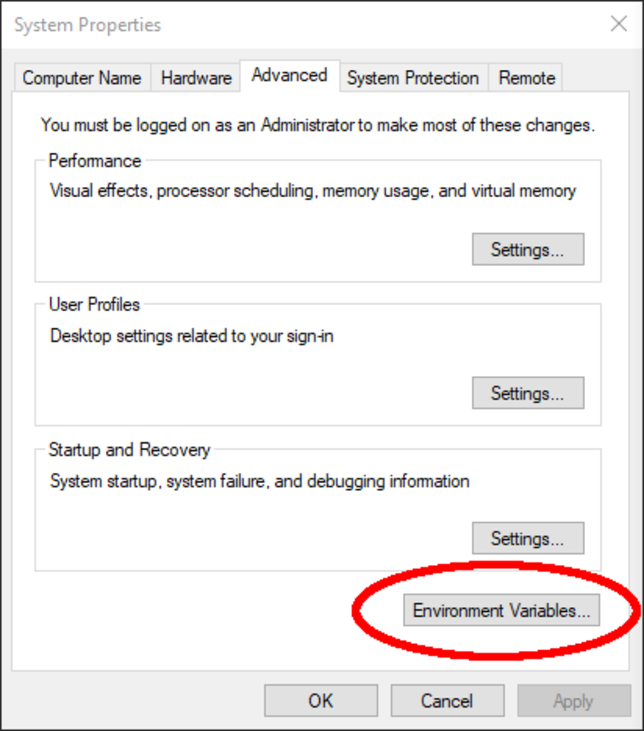
\includegraphics[width=\textwidth]{Figures/win/Win1.pdf}
(a)
\end{center}
\end{minipage}
\begin{minipage}[t]{.29\textwidth}
\begin{center}
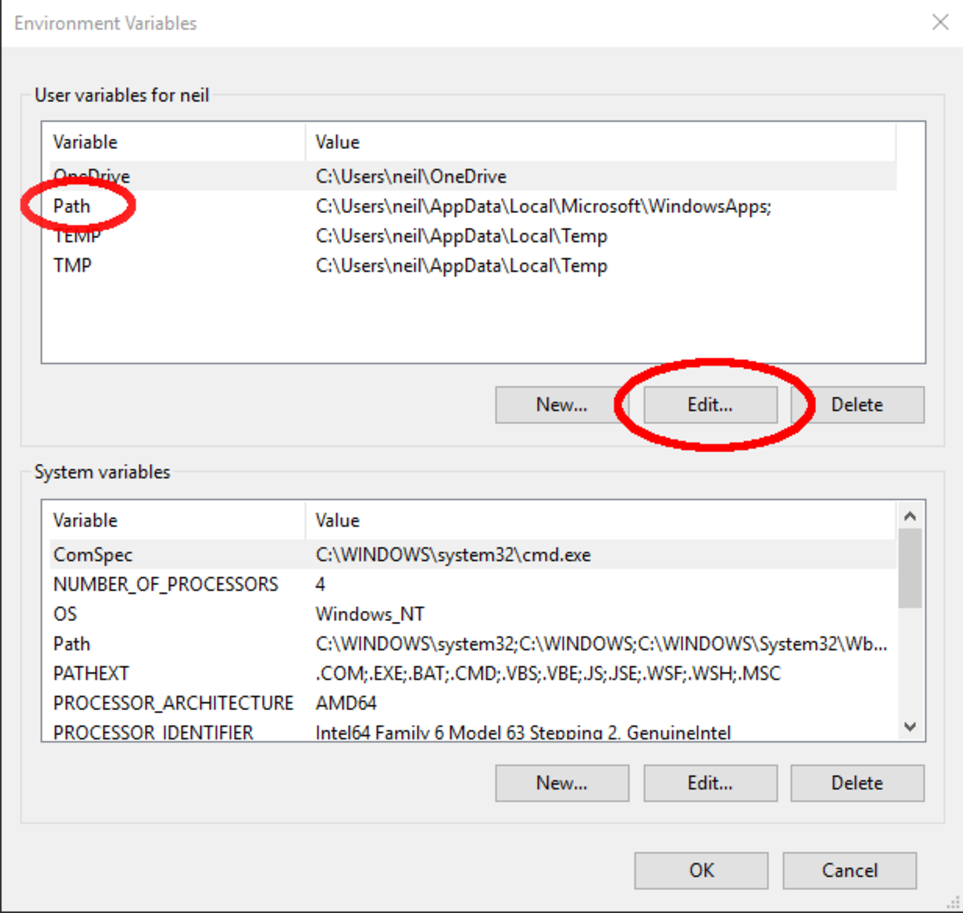
\includegraphics[width=\textwidth]{Figures/win/Win2.pdf}
(b)
\end{center}
\end{minipage}
\begin{minipage}[t]{.29\textwidth}
\begin{center}
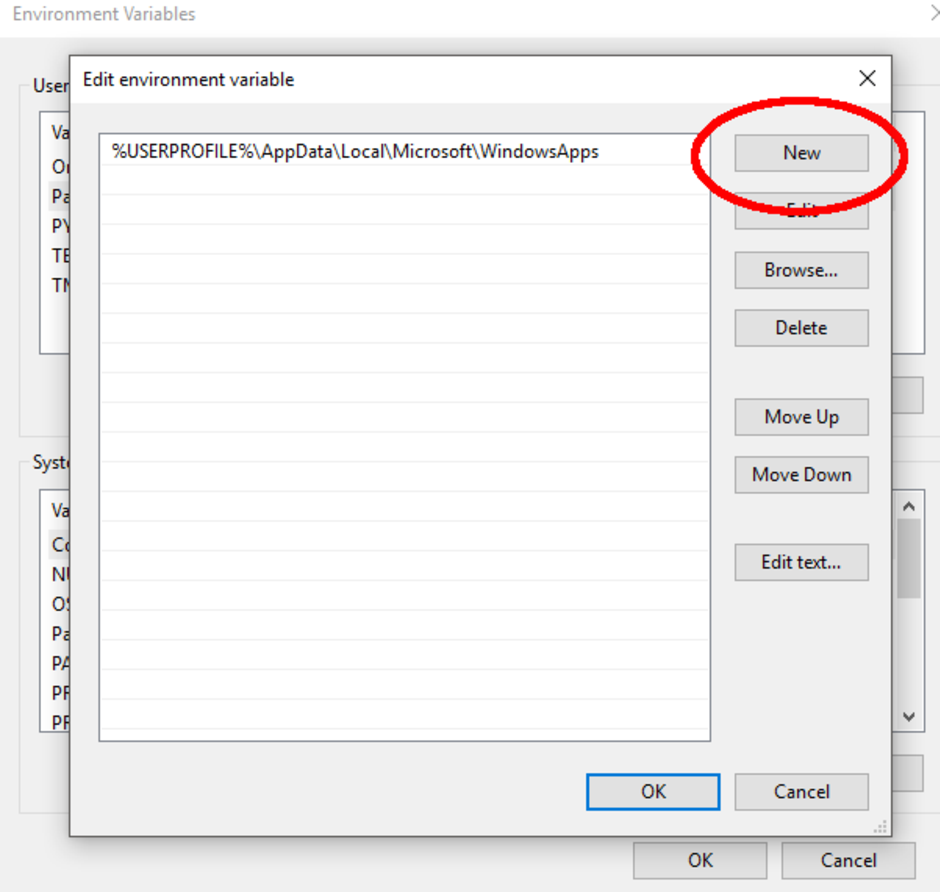
\includegraphics[width=\textwidth]{Figures/win/Win3.pdf}
(c)
\end{center}
\end{minipage}

\begin{minipage}[t]{.29\textwidth}
\begin{center}
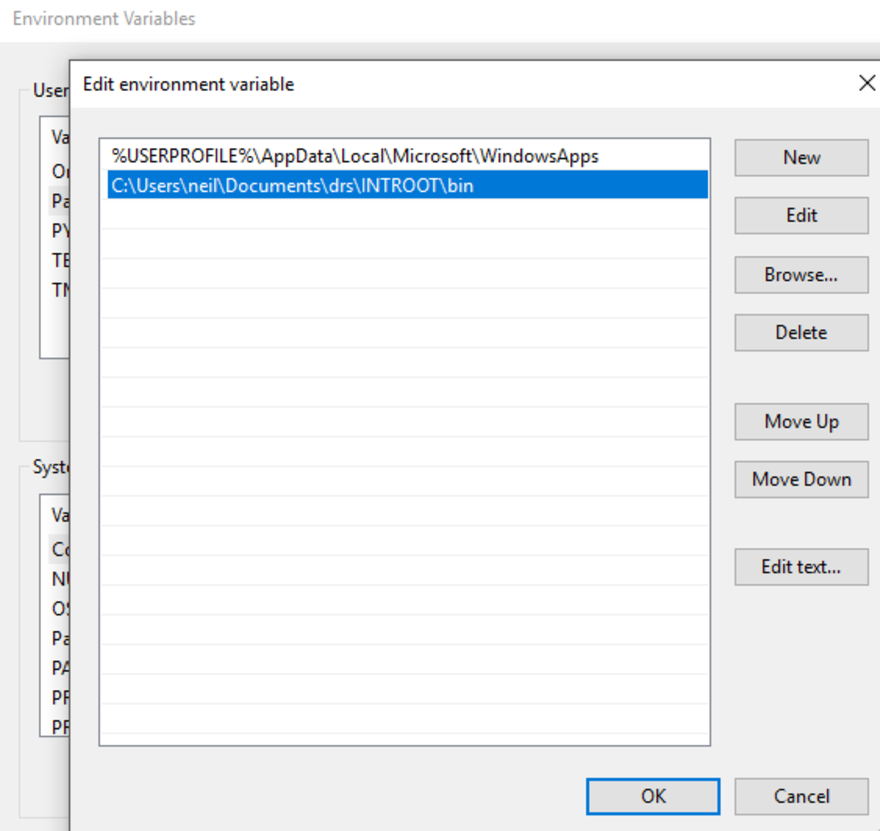
\includegraphics[width=\textwidth]{Figures/win/Win4.pdf}
(d)
\end{center}
\end{minipage}
\begin{minipage}[t]{.29\textwidth}
\begin{center}
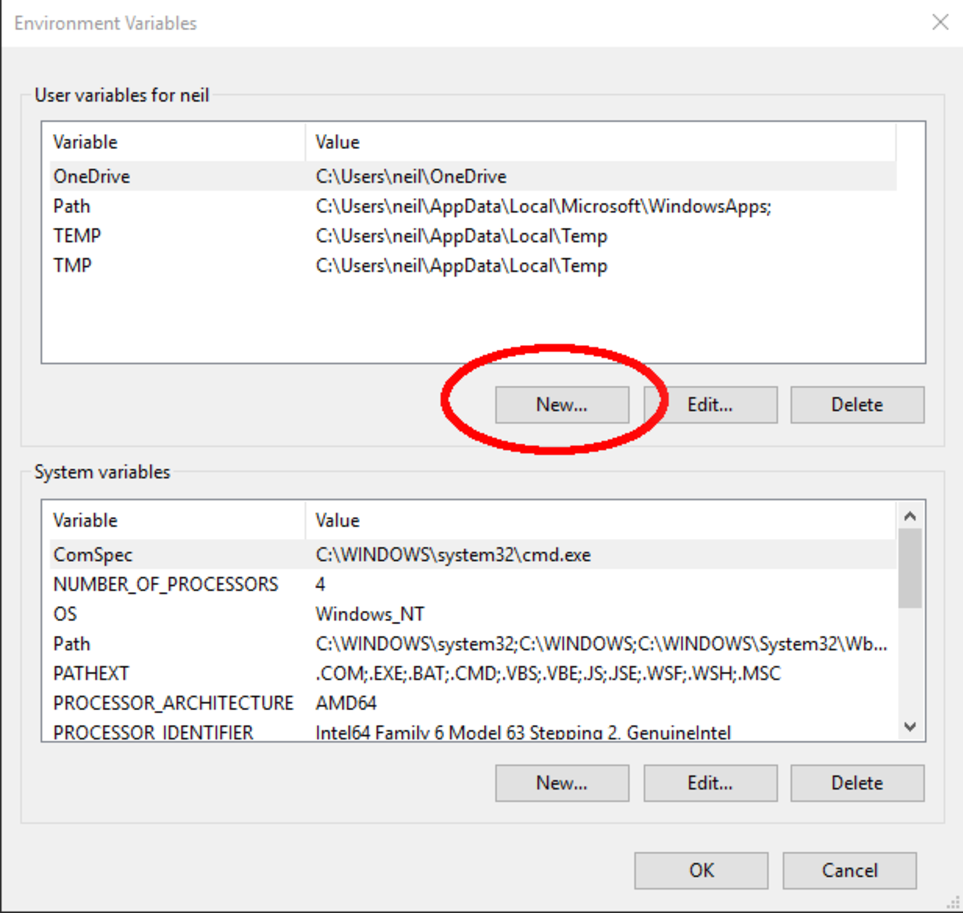
\includegraphics[width=\textwidth]{Figures/win/Win5.pdf}
(e)
\end{center}
\end{minipage}
\begin{minipage}[t]{.29\textwidth}
\begin{center}
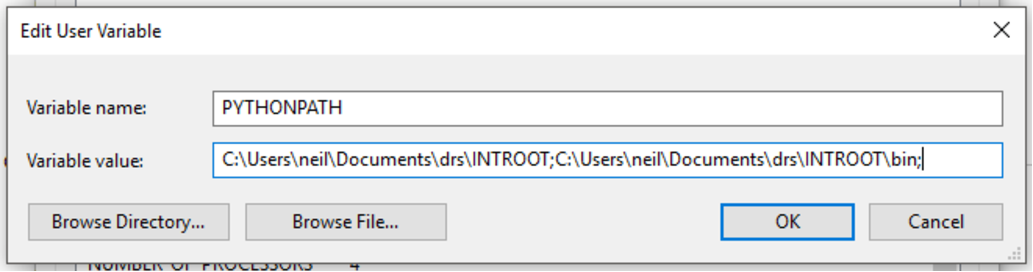
\includegraphics[width=\textwidth]{Figures/win/Win6.pdf}
(f)
\end{center}
\end{minipage}
\end{center}
\caption{(a) Once in ``Advanced system properties'' click ``Environment Variables'' (b) Click ``Path'' and click ``Edit...'' to edit the ``Path'' environmental variable (c) Once in the ``Path'' environmental variable click ``New'' to add a new path (d) Type in the new line to add variable and click ``OK'' (e) Once back in the Enivronmental variable page click ``New'' to add `PYTHONPATH' (f) Set the variable name to ``PYTHONPATH'' and edit the variable value accordingly. \label{figure:screengrabs} }
\end{figure}
\vspace{0.25cm}



%%%%%%%%%%%%%%%%%%%%%%%%%%%%%%%%%%%%%%%%%%%%%%%%%%%%%%%%
%%
\clearpage
\newpage
\section{Setting up the DRS (Windows)}
\label{ch:install:setup_win}
%%
%%%%%%%%%%%%%%%%%%%%%%%%%%%%%%%%%%%%%%%%%%%%%%%%%%%%%%%%

Before running the DRS one must set the data paths. \\

\noindent The `\configtxtfile' file is located in the \InstallDIR in the config folder.

i.e. at \InstallDIR\path{\\config\\}{configtxtfile} \\

\noindent The following keywords \textbf{must} be changed (and must be a valid path):
\begin{thighlight}
\begin{table}[H]
{\footnotesize
\begin{tabular}{p{4cm} p{0.05cm} p{2.5cm} p{0.05cm} p{5.5cm}}
\definevariable{text:drs_root}{TDATA}            & = & \path{C:\\Users\\User\\Documents\\drs\\data}        & / & Define the DATA directory\\
&&&&\\
\definevariable{text:drs_root}{DRS\_ROOT}         & = & \path{C:\\Users\\User\\Documents\\drs\\INTROOT}     & / & Define the installation directory \\
\definevariable{text:drs_data_raw}{DRS\_DATA\_RAW}     & = & \path{C:\\Users\\User\\Documents\\drs\\data\\raw}    & / & Define the folder with the raw data files in \\
\definevariable{text:drs_data_reduc}{DRS\_DATA\_REDUC}   & = & \path{C:\\Users\\User\\Documents\\drs\\data\\reduced} & / & Define the directory that the reduced data should be saved to/read from \\
\definevariable{text:drs_calib_db}{DRS\_CALIB\_DB}     & = & \path{C:\\Users\\User\\Documents\\drs\\data\\calibDB} & / & Define the directory that the calibration files should be saved to/read from \\
\definevariable{text:drs_data_msg}{DRS\_DATA\_MSG}     & = & \path{C:\\Users\\User\\Documents\\drs\\data\\msg}    & / & Define the directory that the log messages are stored in \\
\definevariable{text:drs_data_working}{DRS\_DATA\_WORKING} & = & \path{C:\\Users\\User\\Documents\\drs\\data\\tmp}    & / & Define the working directory \\
\end{tabular}
}
\end{table}
\end{thighlight}
\begin{note}
Note: On windows paths in windows must have a `\textbackslash\textbackslash' also the python files must be open with a valid editor such as sublime text, notepad++, spyder or pycharm for example
\end{note}

\vspace{0.25cm}

\noindent The following keywords can be changed: \\
\begin{thighlight}
\begin{table}[H]
\begin{tabular}{>{\color{red}}l c r c p{5cm}}
\definevariable{text:drs_plot}{DRS\_PLOT}    & = & 1     & / & Whether to show plots \\
\definevariable{text:print_level}{PRINT\_LEVEL} & = & "all" & / & Level at which to print \\
\definevariable{text:log_level}{LOG\_LEVEL}   & = & "all" & / & Level at which to log in log file \\
\end{tabular}
\end{table}

\noindent For the `\definevariable{text:print_level}{PRINT\_LEVEL} and \definevariable{text:log_level}{LOG\_LEVEL} keywords the values are set as follows:
\begin{itemize}
	\item "all" -- prints all events
	\item "info" -- prints info, warning and error events
	\item "warning" -- prints warning and error events
	\item "error" -- print only error events
\end{itemize}
\end{thighlight}



%%%%%%%%%%%%%%%%%%%%%%%%%%%%%%%%%%%%%%%%%%%%%%%%%%%%%%%%
%%
\clearpage
\newpage
\section{Validating Installation on Windows}
\label{ch:install:validating_installwin}
%%
%%%%%%%%%%%%%%%%%%%%%%%%%%%%%%%%%%%%%%%%%%%%%%%%%%%%%%%%

\begin{note}
One must install the DRS (Section \ref{ch:install:install_win}) AND set up the DRS (Section \ref{ch:install:setup}) before validation will be successful.
\end{note}

\noindent In windows there are currently 3 ways to run the RS (running in python/ipython).

\begin{itemize}
\item To validate running from python/ipython from the command line type:
\begin{cmdbox}
python (*\calvalidate*)
ipython (*\calvalidate*)
\end{cmdbox}

\item To validate running from ipython, open ipython and type:
\begin{pythonbox}
@run@ (*\calvalidate*)
\end{pythonbox}

\item To validate running from import from python/ipython, open python/ipython and type:
\begin{pythonbox}
import cal_validate_spirou
cal_validate_spirou.main()
\end{pythonbox}

\end{itemize}

\noindent If validation is successful the following should appear:
\begin{cmdboxprintspecial}
@g
17:34:19.0 -   || *****************************************
17:34:19.0 -   || * SPIROU @(#) Geneva Observatory (0.1.016)
17:34:19.0 -   || *****************************************
17:34:19.0 -   ||(dir_data_raw)      DRS_DATA_RAW=C:\\Users\\User\\Documents\\drs\\data\\raw
17:34:19.0 -   ||(dir_data_reduc)    DRS_DATA_REDUC=C:\\Users\\User\\Documents\\drs\\data\\reduced
17:34:19.0 -   ||(dir_calib_db)      DRS_CALIB_DB=C:\\Users\\User\\Documents\\drs\\data\\calibDB
17:34:19.0 -   ||(dir_data_msg)      DRS_DATA_MSG=C:\\Users\\User\\Documents\\drs\\data\\msg
17:34:19.0 -   ||(print_level)       PRINT_LEVEL=all         %(error/warning/info/all)
17:34:19.0 -   ||(log_level)         LOG_LEVEL=all         %(error/warning/info/all)
17:34:19.0 -   ||(plot_graph)        DRS_PLOT=1            %(def/undef/trigger)
17:34:19.0 -   ||(used_date)         DRS_USED_DATE=undefined
17:34:19.0 -   ||(working_dir)       DRS_DATA_WORKING=C:\\Users\\User\\Documents\\drs\\data\\tmp
17:34:19.0 -   ||                    DRS_INTERACTIVE is not set, running on-line mode
17:34:19.0 -   ||                    DRS_DEBUG is set, debug mode level:1
17:34:19.0 -   ||
17:34:19.0 -   ||Validation successful. DRS installed corrected.
@g
\end{cmdboxprintspecial}

% Chapter 2: Data Architecture
%%%%%%%%%%%%%%%%%%%%%%%%%%%%%%%%%%%%%%%%%%%%%%%%%%%%%%%%
%%
\chapter{Data Architecture}
\label{chapter:data_architecture}
%%
%%%%%%%%%%%%%%%%%%%%%%%%%%%%%%%%%%%%%%%%%%%%%%%%%%%%%%%%

% Chapter 3: Using the DRS
%%%%%%%%%%%%%%%%%%%%%%%%%%%%%%%%%%%%%%%%%%%%%%%%%%%%%%%%
%%
\chapter{Using the DRS}
\label{chapter:using_the_drs}
%%
%%%%%%%%%%%%%%%%%%%%%%%%%%%%%%%%%%%%%%%%%%%%%%%%%%%%%%%%

There are two ways to run the DRS recipes. The first (described in Section \ref{chapter:using_the_drs:direct}) directly calls the code and inputs arguments (either from the command line or from python), the second way is to import the recipes in a python script and define arguments in a call to a function (see Section \ref{chapter:using_the_drs:script}).

%%%%%%%%%%%%%%%%%%%%%%%%%%%%%%%%%%%%%%%%%%%%%%%%%%%%%%%%
%%
\section{Running the DRS recipes directly}
\label{chapter:using_the_drs:direct}
%%
%%%%%%%%%%%%%%%%%%%%%%%%%%%%%%%%%%%%%%%%%%%%%%%%%%%%%%%%

As in Chapter \ref{chapter:installation}, using Linux or \mac one can run DRS recipes from the command line or from python, in windows one is required to be in python before running the scipts. Below we use \calDARK as an example:
\begin{itemize}
\item To run from command line type:
\begin{cmdbox}
(*\calDARK*) YYMMDD Filenames
\end{cmdbox}

\item To run from python/ipython from the command line type:
\begin{cmdbox}
python (*\calDARK*) YYMMDD Filenames
ipython (*\calDARK*) YYMMDD Filenames
\end{cmdbox}

\item To run from ipython, open ipython and type:
\begin{pythonbox}
@run@ (*\calDARK*) YYMMDD Filenames
\end{pythonbox}
\end{itemize}

%%%%%%%%%%%%%%%%%%%%%%%%%%%%%%%%%%%%%%%%%%%%%%%%%%%%%%%%
%%
\section{Running the DRS recipes from a python script}
\label{chapter:using_the_drs:script}
%%
%%%%%%%%%%%%%%%%%%%%%%%%%%%%%%%%%%%%%%%%%%%%%%%%%%%%%%%%

In any operating system one can also import a recipe and call a function to run the code. This is useful in batch operations, timing tests and unit tests for example. Below we use \calDARK as an example:

\begin{pythonbox}
# import the recipe
import cal_DARK_spirou
# define the night folder name
night_name = "20170710"
# define the file(s) to run through the code
files = ['dark_dark02d406.fits']
# run code
cal_validate_spirou.main(night_name=night_name, files=files)
\end{pythonbox}


%%%%%%%%%%%%%%%%%%%%%%%%%%%%%%%%%%%%%%%%%%%%%%%%%%%%%%%%
%%
\section{Working example of the code for SPIRou}
\label{chapter:using_the_drs:working_example}
%%
%%%%%%%%%%%%%%%%%%%%%%%%%%%%%%%%%%%%%%%%%%%%%%%%%%%%%%%%

% ----------------------------------------------
\subsection{Overview}
\label{chapter:using_the_drs:working_example:overview}
% ----------------------------------------------

For this example all files are from:
\begin{cmdbox}
spirou@10.102.14.81:/data/RawImages/H2RG-AT4/AT4-04/2017-07-10_15-36-18/ramps/
\end{cmdbox} 

\noindent following our example data architecture (from Section \ref{ch:install:setup} and shown explicity in Section \ref{ch:data_architecture:folder_layout}) all files should be places in the \definevariable{text:drs_data_raw}{DRS\_DATA\_RAW} (\textcolor{blue}{/drs/data/raw} in our case).

\noindent and we will also need the current WAVE file from here:
\begin{cmdbox}
spirou@10.102.14.81:/data/reduced/DATA-CALIB/spirou_wave_ini3.fits
\end{cmdbox}

\noindent which needs to be placed in the \definevariable{text:drs_calib_db}{DRS\_CALIB\_DB} dirctory (\textcolor{blue}{/drs/data/calibDB} in our case).

\noindent Starting with RAMP files and ending with extracted orders and calculated drifts we need to run six codes:
\begin{enumerate}
\item \calDARK \hfill (See Section \ref{ch:the_recipes:cal_DARK_spirou})
\item \callocRAW ($\times$2) \hfill (See Section \ref{ch:the_recipes:cal_loc_RAW_spirou})
\item \calSLIT \hfill (See Section \ref{ch:the_recipes:cal_SLIT_spirou})
\item \calFFraw ($\times$2) \hfill (See Section \ref{ch:the_recipes:cal_FF_RAW_spirou})
\item (add spirou\_wave\_ini3.fits to calibDB) 
\item \calextractRAWAB and \calextractRAWC (many times) \hfill (See Section \ref{ch:the_recipes:cal_extract_RAW_spirou})
\item \calDRIFTRAW \hfill (See Section \ref{ch:the_recipes:cal_DRIFT_RAW_spirou})
\end{enumerate}





% ----------------------------------------------
\subsection{Run through from command line/python shell (Linux and macOS)}
\label{chapter:using_the_drs:working_example:run_cmd}
% ----------------------------------------------

As long as all codes are excutable (see Section \ref{ch:install:installunix:executable}) one can run all codes from the command line or if not excutable or one has a preference for python one can run the following with `python \{command\}', `ipython \{command\}' or indeed through an interactive ipython session using `run \{command\}'.

\begin{enumerate}

\item run the dark extraction on the `dark\_dark' file:
\begin{cmdbox}
cal_DARK_spirou.py 20170710 dark_dark02d406.fits
\end{cmdbox}

\item run the order localisation on the `dark\_flat' files:
\begin{cmdbox}
cal_loc_RAW_spirou.py 20170710 dark_flat02f10.fits dark_flat03f10.fits dark_flat04f10.fits dark_flat05f10.fits dark_flat06f10.fits
\end{cmdbox}

\item run the order localisation on the `flat\_dark' files:
\begin{cmdbox}
cal_loc_RAW_spirou.py 20170710 flat_dark02f10.fits flat_dark03f10.fits flat_dark04f10.fits flat_dark05f10.fits flat_dark06f10.fits
\end{cmdbox}

\item run the slit calibration on the `fp\_fp' files.
\begin{cmdbox}
cal_SLIT_spirou.py 20170710 fp_fp02a203.fits fp_fp03a203.fits fp_fp04a203.fits
\end{cmdbox}

\item run the flat field creation on the `dark\_flat' files:

\begin{note}
if using same files as above you will get an error message when running the file.

\noindent To solve this open the `\masterCALIBDBfile' file located in \textcolor{blue}{\{DATA\_ROOT\_CALIB\}}. Edit the unix date in the line that begins `TILT' so that it is less than or equal to the unix date on rows `ORDER\_PROFIL\_AB' (i.e. easiest to change it to the date on the `ORDER\_PROFIL\_AB')

\noindent The human date format must match the unix date thus both must be changed if one is modified.

\noindent i.e. the `\masterCALIBDBfile' file should look go from
\begin{textbox}
DARK 20170710 dark_dark02d406.fits 07/10/17/16:37:48 1499704668.0
ORDER_PROFIL_C 20170710 dark_flat02f10_order_profil_C.fits 07/10/17/17:03:50 1499706230.0
LOC_C 20170710 dark_flat02f10_loco_C.fits 07/10/17/17:03:50 1499706230.0
ORDER_PROFIL_AB 20170710 flat_dark02f10_order_profil_AB.fits 07/10/17/17:07:08 1499706428.0
LOC_AB 20170710 flat_dark02f10_loco_AB.fits 07/10/17/17:07:08 1499706428.0
TILT 20170710 fp_fp02a203_tilt.fits @07/10/17/17:25:15 1499707515.0@
\end{textbox}
\noindent to this:
\begin{textbox}
DARK 20170710 dark_dark02d406.fits 07/10/17/16:37:48 1499704668.0
ORDER_PROFIL_C 20170710 dark_flat02f10_order_profil_C.fits 07/10/17/17:03:50 1499706230.0
LOC_C 20170710 dark_flat02f10_loco_C.fits 07/10/17/17:03:50 1499706230.0
ORDER_PROFIL_AB 20170710 flat_dark02f10_order_profil_AB.fits 07/10/17/17:07:08 1499706428.0
LOC_AB 20170710 flat_dark02f10_loco_AB.fits 07/10/17/17:07:08 1499706428.0
TILT 20170710 fp_fp02a203_tilt.fits @07/10/17/17:07:08 1499706428.0@
\end{textbox}
\end{note}

\begin{cmdbox}
cal_FF_RAW_spirou.py 20170710 dark_flat02f10.fits dark_flat03f10.fits dark_flat04f10.fits dark_flat05f10.fits dark_flat06f10.fits
\end{cmdbox}

\newpage

\item Currently we do not create a new wavelength calibration file for this run. Therefore we need one (as stated in the above section). We use the one from here:
\begin{cmdbox}
spirou@10.102.14.81:/data/reduced/DATA-CALIB/spirou_wave_ini3.fits
\end{cmdbox}

\noindent then place it in the \definevariable{text:drs_calib_db}{DRS\_CALIB\_DB} folder. You will also need to edit the `\masterCALIBDBfile' file located in \definevariable{text:drs_calib_db}{DRS\_CALIB\_DB}. 

\noindent Add the folloing line to `\masterCALIBDBfile'
\begin{textbox}
@WAVE 20170710 spirou_wave_ini3.fits 07/10/17/17:03:50 1499706230.0@
\end{textbox}

\noindent and the `master\_calib\_SPIROU.txt' should look like this:
\begin{textbox}
DARK 20170710 dark_dark02d406.fits 07/10/17/16:37:48 1499704668.0
ORDER_PROFIL_C 20170710 dark_flat02f10_order_profil_C.fits 07/10/17/17:03:50 1499706230.0
LOC_C 20170710 dark_flat02f10_loco_C.fits 07/10/17/17:03:50 1499706230.0
ORDER_PROFIL_AB 20170710 flat_dark02f10_order_profil_AB.fits 07/10/17/17:07:08 1499706428.0
LOC_AB 20170710 flat_dark02f10_loco_AB.fits 07/10/17/17:07:08 1499706428.0
TILT 20170710 fp_fp02a203_tilt.fits 07/10/17/17:07:08 1499706428.0
@WAVE 20170710 spirou_wave_ini3.fits 07/10/17/17:03:50 1499706230.0@
\end{textbox}

\item run the extraction files on the `hcone\_dark', `dark\_hcone', `hcone\_hcone', `dark\_dark\_AHC1', `hctwo\_dark', `dark\_hctwo', `hctwo-hctwo', `dark\_dark\_AHC2' and `fp\_fp'  files. For example for the `fp\_fp' files:
\begin{cmdbox}
cal_extract_RAW_spirouAB.py 20170710 fp_fp02a203.fits fp_fp03a203.fits fp_fp04a203.fits
cal_extract_RAW_spirouC.py 20170710 fp_fp02a203.fits fp_fp03a203.fits fp_fp04a203.fits
\end{cmdbox}

\item run the drift calculation on the `fp\_fp' files:
\begin{cmdbox}
@cal_DRIFT_RAW_spirou.py 20170710 @fp_fp02a203.fits fp_fp03a203.fits fp_fp04a203.fits
\end{cmdbox}

\end{enumerate}

% ----------------------------------------------
\clearpage
\newpage
\subsection{Run through python script}
\label{chapter:using_the_drs:working_example:run_python}
% ----------------------------------------------

The process is in the same order as Section \ref{chapter:using_the_drs:working_example:run_cmd}, including changing the date on the `TILT' keyword and adding the `WAVE' line, and adding the wave file to the calibDB folder).

\begin{pythonbox}
import cal_DARK_spirou, cal_loc_RAW_spirou
import cal_SLIT_spirou, cal_FF_RAW_spirou
import cal_extract_RAW_spirou, cal_DRIFT_RAW_spirou
import matplotlib.pyplot as plt
# define constants
NIGHT_NAME = '20170710'
# cal_dark_spirou
files = ['dark_dark02d406.fits']          # set up files
cal_DARK_spirou.main(NIGHT_NAME, files)   # run cal_dark_spirou
plt.close('all')                          # close graphs
# cal_loc_RAW_spirou - flat_dark
files = ['flat_dark02f10.fits', 'flat_dark03f10.fits', 'flat_dark04f10.fits',
         'flat_dark05f10.fits','flat_dark06f10.fits']
cal_loc_RAW_spirou.main(NIGHT_NAME, files)
plt.close('all')
# cal_loc_RAW_spirou - dark_flat
files = ['dark_flat02f10.fits', 'dark_flat03f10.fits', 'dark_flat04f10.fits', 
         'dark_flat05f10.fits', 'dark_flat06f10.fits']
cal_loc_RAW_spirou.main(NIGHT_NAME, files)
plt.close('all')
# cal_SLIT_spirou
files = ['fp_fp02a203.fits', 'fp_fp03a203.fits', 'fp_fp04a203.fits']
cal_SLIT_spirou.main(NIGHT_NAME, files)
plt.close('all')
# cal_FF_RAW_spirou - flat_dark
files = ['flat_dark02f10.fits', 'flat_dark03f10.fits','flat_dark04f10.fits',
         'flat_dark05f10.fits', 'flat_dark06f10.fits']
cal_FF_RAW_spirou.main(NIGHT_NAME, files)
plt.close('all')
# cal_FF_RAW_spirou - dark_flat
files = ['dark_flat02f10.fits', 'dark_flat03f10.fits', 'dark_flat04f10.fits', 
         'dark_flat05f10.fits', 'dark_flat06f10.fits']
cal_FF_RAW_spirou.main(NIGHT_NAME, files)
plt.close('all')
# cal_extract_RAW_spirou - fp_fp AB
files = ['fp_fp02a203.fits', 'fp_fp03a203.fits', 'fp_fp04a203.fits']
cal_extract_RAW_spirou.main(NIGHT_NAME, files, 'AB')
plt.close('all')
# cal_extract_RAW_spirou - fp_fp C
files = ['fp_fp02a203.fits', 'fp_fp03a203.fits', 'fp_fp04a203.fits']
cal_extract_RAW_spirou.main(NIGHT_NAME, files, 'C')
plt.close('all')
# test cal_DRIFT_RAW_spirou
files = ['fp_fp02a203.fits', 'fp_fp03a203.fits', 'fp_fp04a203.fits']
cal_DRIFT_RAW_spirou.main(NIGHT_NAME, files)
plt.close('all')

\end{pythonbox}


% Chapter 4: Changelog (This version and AT-4)
%%%%%%%%%%%%%%%%%%%%%%%%%%%%%%%%%%%%%%%%%%%%%%%%%%%%%%%%
%%
\chapter{Summary of changes (AT-4)}
\label{ch:changelog}
%%
%%%%%%%%%%%%%%%%%%%%%%%%%%%%%%%%%%%%%%%%%%%%%%%%%%%%%%%%

Below we describe breifly the main differences from AT-4 build.

%%%%%%%%%%%%%%%%%%%%%%%%%%%%%%%%%%%%%%%%%%%%%%%%%%%%%%%%
%%
\section{General}
%%
%%%%%%%%%%%%%%%%%%%%%%%%%%%%%%%%%%%%%%%%%%%%%%%%%%%%%%%%
\begin{itemize}

\item all recipes main body of code is now in a \definevariable{\progMAIN} function and this function is called in \definevariable{\MAIN} part of the code (the part that executes at run time). This allows recipes to be called as functions as well as being called as a standalone code or from the command line. i.e. for \calDARK:
	\begin{pythonbox}
	import cal_DARK_spirou
	    
	files = ['dark_dark02d406.fits']
	night_name = '20170710'
	cal_DARK_spirou.main(night_name=night_name, files=files)
	\end{pythonbox}
	will run the exact same procedure as:
	\begin{bashbox}
	cal_DARK_spirou.py 201707 dark_dark02d406.fits
	\end{bashbox}

\item \definevariable{WLOG} function overhal (now in \definevariable{\spirouLog.logger()}) but aliased in most codes back to \definevariable{WLOG}. This means one can use the same functionality as before:
	\begin{pythonbox}
	WLOG("warning", "program", "message")
	\end{pythonbox}
	However now when "error" is called an automatic exit routine is run (therefore there is no need for sys.exit after a WLOG("error", "", "") call).

\item execution of pythonstartup codes removed and replaced with functions

\item loading of many variables into python memory replaced with call to need dictionary object (parameter dictionary). Parameter dictionary is a custom dictionary object that as well as storing key and value pairs also can set a source for each key in the dictionary (hence the developer will always know where a variable was defined, if used correctly)

\item All hard coded constants removed from running code and moved to configuration files, all variables have been described, noted their new definition locations and where they are used in the recipes and codes (see Section \ref{ch:variables}). This has allowed (and will allow) variables to either be public (i.e. in a location easily accessible by the user) or to be private (in files stored within the module). We can make many specific configuration files or a few, depending on which we deem best.

\item Custom exception: \definevariable{ConfigError} and \definevariable{ConfigException} - designed specifically to be used with the WLOG() function 

\item moved core functions used in multiple recipes to sub-modules

\item all plotting taken out of main codes (call to specific sub-module)

\end{itemize}

%%%%%%%%%%%%%%%%%%%%%%%%%%%%%%%%%%%%%%%%%%%%%%%%%%%%%%%%
%%
\section{The cal\_DARK\_spirou recipe}
\label{ch:changelog:At4:cal_DARK_spirou}
%%
%%%%%%%%%%%%%%%%%%%%%%%%%%%%%%%%%%%%%%%%%%%%%%%%%%%%%%%%

\begin{itemize}

\item dark measurement moved to function \definevariable{\spirouImage.MeasureDark} (for clarity). This is, in part, due to the repetition of code for ``Whole det'', ``Blue part'' and ``Red part''.

\item all plotting moved to internal functions (for clarity)
	\begin{itemize}
    \item \definevariable{\spirouPlot.darkplot\_image\_and\_regions} for the image/region plot
    \item \definevariable{\spirouPlot.darkplot\_datacut} for the DARK cutlimit plot
    \item \definevariable{\spirouPlot.darkplot\_histograms} for the histogram plots 
    \end{itemize}

\item histogram plot updated, original plot plotted bin centers as a smooth peak, simple modification to make sure histogram bars are present
    
\item writing of data is sped up by caching all HEADER keys and writing to file once with the write of the data.

\item speed up
	\begin{itemize}
	\item AT-4 v44: 4.881 seconds
	\item py3: 1.890 seconds
	\end{itemize}

\end{itemize}

%%%%%%%%%%%%%%%%%%%%%%%%%%%%%%%%%%%%%%%%%%%%%%%%%%%%%%%%
%%
\section{The cal\_loc\_RAW\_spirou recipe}
\label{ch:changelog:At4:cal_loc_RAW_spirou}
%%
%%%%%%%%%%%%%%%%%%%%%%%%%%%%%%%%%%%%%%%%%%%%%%%%%%%%%%%%

\begin{itemize}

\item added function to convert from ADU/s to electrons \definevariable{\spirouImage.ConvertToE}
    
\item added function to flip image \definevariable{\spirouImage.FlipImage}

\item smoothed image (by a box) is now in a function (creates order\_profile)
	\begin{itemize}
	\item added different way to calculate order\_profile - currently set to 'manual' be default
	\item \definevariable{\spirouLOCOR.BoxSmoothedImage} 
	\item Instead of manually working out the mean for each box you convolve the weighted image with a tophat function and the weights with a topcat function and then divide the two.
	\item This gives approximately the same result (with small deviations due to the FT of a topcat function not being perfect).
	\item The function can be turned back to the original manual mode by using `mode='manual'' but is slower (by a factor of $\sim\times$8)
	\end{itemize}

\item added storage dictionary to store (and pass around) all variables created `loc' - a Parameter dictionary (thus source can be set for all variables to keep track of them)

\item added function to measure background and get central pixel positions \definevariable{\spirouLOCOR.MeasureBkgrdGetCentPixs}

\item debug plot added to plot the minimum of `ycc' and `ic\_locseuil' \definevariable{\spirouPlot.sPlt.debug\_locplot\_min\_ycc\_loc\_threshold}

\item added function for locating central position (previously \definevariable{\spirouLOCOR.poscolc}) - currently set to 'manual' be default
    \begin{itemize}
    \item \definevariable{\spirouLOCOR.LocateCentralOrderPositions} 
    \item  Instead of manually working out the starts and ends of each order (with while loops) convolves a mask of cvalues > threshold with a top-hat (size=3) function such that all edges are found
    \item i.e. `[False, True, True]` or `[True, True, False]` give a different value than `[True, True, True]` or `[False, False, False]` or `[False, False, True]`
    \item i.e. the convolution gives the sum of three elements, thus selected those elements with a sum of 2 give our edges
    \item The function can be turned back to the original 'manual' mode by using `mode='manual` but is slower (by a factor of x2)
	\end{itemize}

\item debug plot added to plot the image above saturation threshold \definevariable{\spirouPlot.locplot\_im\_sat\_threshold}
        
\item moved `ctro`,`sigo`,`ac`,`ass` etc into loc (for storage and ease of use)        
        
\item the fit across each order has been split into functions
    \begin{itemize}
	\item the initial fit is done by \definevariable{\spirouLOCOR.InitialOrderFit}
	\item This initial fit takes in the plotting args and thus as order is fit the fit is piped on to plot via \definevariable{\spirouPlot.locplot\_order}
	\item the sigma clipping fit is done by \definevariable{\spirouLOCOR.SigClipOrderFit}
	\item kind is used to change between 'center' and 'fwhm' fits (thus function is reused in both cases), kind will do the tiny bits of code which are different for each fit
	\item all fit parameters are loaded into the `loc` parameter dictionary
	\end{itemize}

\item plot of order number against rms is move to \definevariable{\spirouPlot.locplot\_order{\hskip 0pt}\_number\_against\_rms}

\item function created to add the 2Dlist (i.e. the coefficients) to hdict (the dictionary used to save keys to so that we only write to the fits file once)

\item superimposed fit on the image is pushed into a function, this is many times faster than before - due to optimisation, \definevariable{\spirouLOCOR.imageLocSuperimp}

\item Writing of fits file cleaned up (header keywords written during data write)

\item speed up
	\begin{itemize}
	\item AT-4 v44: 5.697 seconds
	\item py3:  2.255 seconds
    \end{itemize}

\end{itemize}

%%%%%%%%%%%%%%%%%%%%%%%%%%%%%%%%%%%%%%%%%%%%%%%%%%%%%%%%
%%
\section{The cal\_SLIT\_spirou recipe}
\label{ch:changelog:At4:cal_SLIT_spirou}
%%
%%%%%%%%%%%%%%%%%%%%%%%%%%%%%%%%%%%%%%%%%%%%%%%%%%%%%%%%

\begin{itemize}
\item added storage dictionary to store (and pass around) all variables created `loc` - a Parameter dictionary (thus source can be set for all variables to keep track of them)

\item Retrieval of coefficients from `\_loco\_` file moved to \definevariable{\spirouLOCOR.GetCoeffs}

\item Tilt finding is moved to function \definevariable{\spirouImage.GetTilt}

\item Fitting the tilt is moved to function \definevariable{\spirouImage.FitTilt}

\item selected order plot moved to \definevariable{\spirouPlot.slit\_sorder\_plot}

\item slit tilt angle and fit plot moved to \definevariable{\spirouPlot.slit\_tilt\_angle\_and\_fit\_plot}

\item Writing of fits file cleaned up (header keywords written during data write)

\item speed up
	\begin{itemize}
	\item AT-4 v44: 11.071 seconds
	\item py3: 4.386 seconds
    \end{itemize}

\end{itemize}

%%%%%%%%%%%%%%%%%%%%%%%%%%%%%%%%%%%%%%%%%%%%%%%%%%%%%%%%
%%
\section{The cal\_FF\_RAW\_spirou recipe}
\label{ch:changelog:At4:cal_FF_RAW_spirou}
%%
%%%%%%%%%%%%%%%%%%%%%%%%%%%%%%%%%%%%%%%%%%%%%%%%%%%%%%%%

\begin{itemize}
\item added function to replace measure\_bkgr\_FF, but incomplete (not currently used) would need to convert interpol.c to python (spline fitting)

\item added storage dictionary to store (and pass around) all variables created `loc` - a Parameter dictionary (thus source can be set for all variables to keep track of them)

\item Created function to read TILT file from calibDB (replaces `readkeyloco`)
	\begin{itemize}
    \item \definevariable{\spirouImage.ReadTiltFile}
    \item takes in header dictionary from `fitsfilename` in order to avoid re-opening FITS rec (acqutime used in calibDB to get max\_time of calibDB entry) 
    \end{itemize}
\item Created function to read order profile (replaces `read\_data\_raw` + pre-amble)
	\begin{itemize}
	\item \definevariable{\spirouImage.ReadOrderProfile}
	\item takes in header dictionary from `fitsfilename` in order to avoid re-opening FITS rec (acqutime used in calibDB to get max\_time of calibDB entry) 
    \end{itemize}
\item Used \definevariable{\spirouLOCOR.GetCoeffs} to get the coefficients from file

\item Created merge coefficients function to perform AB coefficient merge \definevariable{\spirouLOCOR.MergeCoefficients}
    
\item Updated extraction function \definevariable{\spirouEXTOR.ExtracTiltWeightOrder2} - much faster as takes many of the calculations outside the pixel loop
	\begin{itemize}
	\item i.e. calculating the pixel contribution due to tilt in array `ww`
	\item `ww` is constant for an order, thus doesn't need to be worked out for each pixel in one order, just the multiplication between ww and the image
	\item up to 8 times faster with these improvements
    \end{itemize}
\item `e2ds`, `SNR`, `RMS`, `blaze` and `flat` are stored in `loc` parameter dictionary

\item Plotting code moved to \definevariable{\spirouPlot} functions

\item Writing of fits file cleaned up (header keywords written during data write)

\item QC (max\_signal $>$ qc\_max\_signal $\times$ nbframes) moved to end, however in old code it is not used as a failure criteria so also not used to fail in new code

\item speed up
	\begin{itemize}
	\item AT-4 v44: 25.962 seconds
	\item py3: 4.675 seconds
    \end{itemize}

\end{itemize}

%%%%%%%%%%%%%%%%%%%%%%%%%%%%%%%%%%%%%%%%%%%%%%%%%%%%%%%%
%%
\section{The cal\_extract\_RAW\_spirou recipes}
\label{ch:changelog:At4:cal_extract_RAW_spirou}
%%
%%%%%%%%%%%%%%%%%%%%%%%%%%%%%%%%%%%%%%%%%%%%%%%%%%%%%%%%

\begin{itemize}
\item Merged \definevariable{cal\_extract{\hskip 0pt}\_RAW\_spirouAB}, \definevariable{cal\_extract{\hskip 0pt}\_RAW\_spirouC} and \definevariable{cal\_extract\_RAW{\hskip 0pt}\_spirouALL} can still access \definevariable{cal\_extract{\hskip 0pt}\_RAW\_spirouAB} and \definevariable{cal\_extract{\hskip 0pt}\_RAW\_spirouC} but instead of being modified copies of the code they are just wrappers for \definevariable{cal\_extract\_RAW{\hskip 0pt}\_spirou.py} (i.e. they forward the fiber type)

\item added storage dictionary to store (and pass around) all variables created `loc` - a Parameter dictionary (thus source can be set for all variables to keep track of them)

\item Created function to read TILT file from calibDB (replaces `readkeyloco`)
    \begin{itemize}
	\item \definevariable{\spirouImage.ReadTiltFile}
	\item takes in header dictionary from `fitsfilename` in order to avoid re-opening FITS rec (acqutime used in calibDB to get max\_time of calibDB entry) 
    \end{itemize}

\item Created function to read WAVE file from calibDB (replaces `read\_data\_raw(`)
    \begin{itemize}
	\item \definevariable{\spirouImage.ReadWaveFile}
	\item takes in header dictionary from `fitsfilename` in order to avoid re-opening FITS rec (acqutime used in calibDB to get max\_time of calibDB entry) 
    \end{itemize}

\item Used \definevariable{\spirouLOCOR.GetCoeffs} to get the coefficients from file

\item Created function to read order profile (replaces `read\_data\_raw` + pre-amble)
    \begin{itemize}
	\item \definevariable{\spirouImage.ReadOrderProfile}
	\item takes in header dictionary from `fitsfilename` in order to avoid re-opening FITS rec (acqutime used in calibDB to get max\_time of calibDB entry) 
    \end{itemize}

\item Created merge coefficients function to perform AB coefficient merge \definevariable{\spirouLOCOR.MergeCoefficients}

\item New structures above replace the need for specific fiber sections ('AB', 'C', 'A', 'B') (In \definevariable{cal\_extract{\hskip 0pt}\_RAW\_spirouALL} and individual setups for \definevariable{cal\_extract{\hskip 0pt}\_RAW\_spirouAB} and \definevariable{cal\_extract{\hskip 0pt}\_RAW\_spirouC})

\item all extraction functions passed into \definevariable{spirouEXTOR} to wrapper functions (\definevariable{\spirouEXTOR.ExtractOrder}, \definevariable{\spirouEXTOR.ExtractTiltOrder}, \definevariable{\spirouEXTOR.ExtractTiltWeightOrder} and \definevariable{\spirouEXTOR.ExtractWeightOrder}) these are then run into \definevariable{\spirouEXTOR.ExtractionWrapper} and processed accordingly

\item Added a timing string (to record timings of all extraction processes) use `print(timing))` to view
    
\item `e2ds` and `SNR` stored in `loc`

\item Plotting code moved to \definevariable{\spirouPlot} functions

\item Writing of fits file cleaned up (header keywords written during data write)

\item QC (max\_signal $>$ qc\_max\_signal $\times$ nbframes) moved to end, however in old code it is not used as a failure criteria so also not used to fail in new code

\item speed up
	\begin{itemize}
	\item AT-4 v44: 60.852
	\item py3: 8.694

	\item Extraction timing Py3:
		\begin{itemize}
		\item ExtractOrder = 0.025 s
		\item ExtractTiltOrder = 0.060 s
		\item ExtractTiltWeightOrder = 0.141 s
		\item ExtractWeightOrder = 0.070 s
         \end{itemize}

	\item Extraction timing AT-4 v46:
		\begin{itemize}
		\item ExtractOrder (Fortran) = 0.019 s
		\item ExtractOrder (Py2) = 0.085 s
		\item ExtractTiltOrder = 0.766 s
		\item ExtractTiltWeightOrder = 0.840 s
		\item ExtractWeightOrder = 0.156 s
         \end{itemize}

	\item Speed increase (Py3 over AT-4 v46)
		\begin{itemize}
		\item ExtractOrder (Py3 $\rightarrow$ Fortran) = slower    x 1.3 times slower
		\item ExtractOrder (Py3 $\rightarrow$ Py) = faster     x 3.4 times faster
		\item ExtractTiltOrder (Py3 $\rightarrow$ Py = faster     x12.9 times faster
		\item ExtractTiltWeightOrder (Py3 $\rightarrow$ Py) = faster    x6.0 times faster
		\item ExtractWeightOrder (Py3 $\rightarrow$ Py) = faster    x2.2 times faster
		\end{itemize}

	\end{itemize}

\end{itemize}


%%%%%%%%%%%%%%%%%%%%%%%%%%%%%%%%%%%%%%%%%%%%%%%%%%%%%%%%
%%
\section{The cal\_DRIFT\_RAW\_spirou recipe}
\label{ch:changelog:At4:cal_DRIFT_RAW_spirou}
%%
%%%%%%%%%%%%%%%%%%%%%%%%%%%%%%%%%%%%%%%%%%%%%%%%%%%%%%%%

\begin{itemize}
\item acqtime (bjdref) got from header using \definevariable{\spirouImage.GetAcqTime}
	\begin{itemize}
	\item can be used to get both `human` readible and `unix` time (use key kind=`human` or kind=`unix)
	\end{itemize}

\item Created function to read TILT file from calibDB (replaces `readkeyloco`)
	\begin{itemize}
	\item \definevariable{\spirouImage.ReadTiltFile}
	\item takes in header dictionary from `fitsfilename` in order to avoid re-opening FITS rec (acqutime used in calibDB to get max\_time of calibDB entry) 
	\end{itemize}

\item Created function to read WAVE file from calibDB (replaces `read\_data\_raw(`)
	\begin{itemize}
	\item \definevariable{\spirouImage.ReadWaveFile}
	\item takes in header dictionary from `fitsfilename` in order to avoid re-opening FITS rec (acqutime used in calibDB to get max\_time of calibDB entry) 
	\end{itemize}

\item Used \definevariable{\spirouLOCOR.GetCoeffs} to get the coefficients from file

\item Created function to read order profile (replaces `read\_data\_raw` + pre-amble)
	\begin{itemize}
	\item \definevariable{\spirouImage.ReadOrderProfile}
	\item takes in header dictionary from `fitsfilename` in order to avoid re-opening FITS rec (acqutime used in calibDB to get max\_time of calibDB entry) 
	\end{itemize}

\item new extraction (see \calextractRAW above).

\item delta RV RMS calculation in \definevariable{\spirouRV.DeltaVrms2D}
	\begin{itemize}
	\item where arguments are `speref` and `wave` (stored in `loc`)
	\item where keyword arguments are `sigdet`, `size` and `threshold` (stored in p)
	\end{itemize}

\item all functionality to do with listing files moved to \definevariable{\spirouImage{\hskip 0pt}.GetAllSimilarFiles} - no need for "alphanumeric short"/"nice sort" - `np.sort(x)` does this
    
\item Renormlisation and cosmics correction in \definevariable{\spirouRV.ReNormCosmic2D}
	\begin{itemize}
	\item where arguments are `speref` and `spe` (stored in `loc`)
	\item where keyword arguments are `cut`, `size` and `threshold` (stored in p)
	\end{itemize}

\item RV drift calculated
	\begin{itemize}
	\item \definevariable{\spirouRV.CalcRVdrift2D}
	\item where arguments are `speref`, `spen` and `wave` (`speref` and `spen` stored in loc)
	\item where keyword arguments are `sigdet`, `size` and `threshold` (stored in p)
	\end{itemize}

\item added an option (drift\_type\_e2ds) to decide between getting drift using a weighted mean or using a median (to combine all orders)

\item `drift`, `errdrift`, `deltatime`, `mdrift`, `merrdrift` stored in loc

\item Writing of fits file cleaned up (header keywords written during data write)

\item speed up
	\begin{itemize}
	\item AT-4 v44: 22.556 s
	\item py3:  8.143 s
	\end{itemize}

\end{itemize}


%%%%%%%%%%%%%%%%%%%%%%%%%%%%%%%%%%%%%%%%%%%%%%%%%%%%%%%%
%%
\section{The cal\_BADPIX\_spirou recipe}
\label{ch:changelog:At4:cal_BADPIX_spirou}
%%
%%%%%%%%%%%%%%%%%%%%%%%%%%%%%%%%%%%%%%%%%%%%%%%%%%%%%%%%

\begin{itemize}
	\item loading of custom arguments moved to \definevariable{\spirouStartup.GetCustomFromRuntime}

	\item loading of files moved to \definevariable{\spirouImage.ReadImage}

	\item normalising flat and median of flat moved to \definevariable{\spirouImage.NormMedianFlat}

	\item locating bad pixels moved to \definevariable{\spirouImage.LocateBadPixels}

	\item instead of taking the 90th pixel in flattened meadian flat image now work out the 90th percentile of finite values (will lead to a slightly more correct normalisation value)

	\item Writing of fits file cleaned up (header keywords written during data write)
\end{itemize}


%%%%%%%%%%%%%%%%%%%%%%%%%%%%%%%%%%%%%%%%%%%%%%%%%%%%%%%%
%%
\section{The cal\_DRIFT\_RAW\_spirou recipe}
\label{ch:changelog:At4:cal_DRIFT_RAW_spirou}
%%
%%%%%%%%%%%%%%%%%%%%%%%%%%%%%%%%%%%%%%%%%%%%%%%%%%%%%%%%

\begin{itemize}
\item loading of custom arguments for reference file

\item acqtime (bjdref) got from header using \definevariable{\spirouImage.GetAcqTime}
	\begin{itemize}
	\item can be used to get both `human` readible and `unix` time (use key kind=`human` or kind=`unix)
	\end{itemize}

\item Created function to read TILT file from calibDB (replaces `readkeyloco`)
	\begin{itemize}
	\item \definevariable{\spirouImage.ReadTiltFile}
	\item takes in header dictionary from `fitsfilename` in order to avoid re-opening FITS rec (acqutime used in calibDB to get max\_time of calibDB entry) 
	\end{itemize}

\item Created function to read WAVE file from calibDB (replaces `read\_data\_raw(`)
	\begin{itemize}
	\item \definevariable{\spirouImage.ReadWaveFile}
	\item takes in header dictionary from `fitsfilename` in order to avoid re-opening FITS rec (acqutime used in calibDB to get max\_time of calibDB entry) 
	\end{itemize}

\item delta RV RMS calculation in \definevariable{\spirouRV.DeltaVrms2D}
	\begin{itemize}
	\item where arguments are `speref` and `wave` (stored in `loc`)
	\item where keyword arguments are `sigdet`, `size` and `threshold` (stored in p)
	\end{itemize}

\item all functionality to do with listing files moved to \definevariable{\spirouImage{\hskip 0pt}.GetAllSimilarFiles} - no need for "alphanumeric short"/"nice sort" - `np.sort(x)` does this
    
\item Renormlisation and cosmics correction in \definevariable{\spirouRV.ReNormCosmic2D}
	\begin{itemize}
	\item where arguments are `speref` and `spe` (stored in `loc`)
	\item where keyword arguments are `cut`, `size` and `threshold` (stored in p)
	\end{itemize}

\item RV drift calculated
	\begin{itemize}
	\item \definevariable{\spirouRV.CalcRVdrift2D}
	\item where arguments are `speref`, `spen` and `wave` (`speref` and `spen` stored in loc)
	\item where keyword arguments are `sigdet`, `size` and `threshold` (stored in p)
	\end{itemize}

\item added an option (drift\_type\_e2ds) to decide between getting drift using a weighted mean or using a median (to combine all orders)

\item `drift`, `errdrift`, `deltatime`, `mdrift`, `merrdrift` stored in loc

\item Writing of fits file cleaned up (header keywords written during data write)

\item new functions to save to .tbl format (\spirouImage.MakeTable and \spirouImage.WriteTable)

\item speed up
	\begin{itemize}
	\item 
	\item 
	\end{itemize}

\end{itemize}

% Chapter 5: Coding rules and standardisation practises
%%%%%%%%%%%%%%%%%%%%%%%%%%%%%%%%%%%%%%%%%%%%%%%%%%%%%%%%
%%
\chapter{Coding style and standardization}
\label{ch:rules}
%%
%%%%%%%%%%%%%%%%%%%%%%%%%%%%%%%%%%%%%%%%%%%%%%%%%%%%%%%%

To keep the code neat, tidy, consistent and professional the following sections suggest guideline by which the DRS should conform to.

%%%%%%%%%%%%%%%%%%%%%%%%%%%%%%%%%%%%%%%%%%%%%%%%%%%%%%%%
%%
\section{PEP 8 - A style guide for python code}
\label{ch:rules:pep8}
%%
%%%%%%%%%%%%%%%%%%%%%%%%%%%%%%%%%%%%%%%%%%%%%%%%%%%%%%%%

PEP 8 is a style guide for python it lays out a specific way to format python code, a full guide can be found here: \url{https://www.python.org/dev/peps/pep-0008/} but the following summarizes the main points used in the DRS.

\begin{itemize}
	\item Code lay-out
	\begin{itemize}
		\item 4 spaces per indentation level (spaces not tabs)
		\item Continuation lines should align wrapped elements
		\item Maximum line length of 79 characters
		\item Surround top-level functions and class definitions with two blank lines (methods with one blank line and all other code with one blank line maximum)
		\item imports should usually be on separate lines
	\end{itemize}

	\item White space in expressions and statements
	\begin{itemize}
		\item No white spaces immediately inside parentheses, brackets or braces
		\item No white spaces immediately before a comma, semicolon, or colon (exception for slicing)
		\item No white spaces immediately before the open parenthesis that starts the argument list of a function call
		\item No white spaces immediately before the open parenthesis that starts an indexing or slicing
		\item Exactly one white space around an assignment (or other) operator
		\item No space around the = sign when used to indicate a keyword argument or a default parameter value
		\item Avoid compound statements (multiple statements on the same line)
	\end{itemize}

	\item Comments
	\begin{itemize}
		\item Comments should start with a \# and be followed by a single white space
		\item In-line comments should be used sparingly
		\item All functions, classes and methods should have a valid document string (see here: \url{https://www.python.org/dev/peps/pep-0257})
	\end{itemize}

	\item Naming conventions
	\begin{itemize}
		\item Never use lower-case letter el `l', upper-case letter `oh' `O', or upper-case letter `eye' `I' as single character variables names
		\item Class Names should normally use CamelCase (words should be Capitalized)
		\item Functions names should be lower-case with words separated by underscores as necessary (same is true for global variable names)
		\item Constants defined on a module level should be written in capital letters with underscores separating words
	\end{itemize}

\end{itemize}


%%%%%%%%%%%%%%%%%%%%%%%%%%%%%%%%%%%%%%%%%%%%%%%%%%%%%%%%
%%
\section{DRS specific style and standardization}
\label{ch:rules:drs_specific}
%%
%%%%%%%%%%%%%%%%%%%%%%%%%%%%%%%%%%%%%%%%%%%%%%%%%%%%%%%%

In addition to PEP-8 we stick to some extra style and standardization points, these include some custom objects to help the ease of development and user experience.

% -------------------------------------------------------
\subsection{Functions from sub-modules}
\label{ch:rules:drs_specific:sub-module_functions}
% -------------------------------------------------------

Unlike `normal' functions these are written in CamelCase without underscores between words. This is done to distinguish them from standard functions. They are always defined in a module (or sub-modules) \INIT\, code and are essentially public aliases to module level code. An example is presented below.

\begin{pythonbox}
# --------------------------
# in the module file spirouMath.py
# --------------------------
def add_x_to_y(x, y):
	"""
	Returns the summation of x and y
	:param x: float, the first term to add
	:param y: float, the second term to add
	:return z: float, the summation of x and y
	"""
	# add x to y
	z = x + y
	# return z
	return z

# --------------------------
# in the __init__ file for spirouCore
# --------------------------
# import from local code
from . import spirouMath
# publicly defined alias to local code function
AddXtoY = spirouMath.add_x_to_y

# --------------------------
# in the recipe
# --------------------------
# import sub-module
from SpirouDRS import spirouCore
# set up constants
x = 4.123
y = 5.234
# add via function
z = spirouCore.AddXtoY(x, y)
\end{pythonbox}


% -------------------------------------------------------
\clearpage
\newpage
\subsection{The logger (WLOG)}
\label{ch:rules:drs_specific:logger}
% -------------------------------------------------------

As in previous version of the DRS the printing and logging is controlled by a function. In this version of the DRS this is in \spirouLog.logger but in most recipes/modules this is aliased to \WLOG. The \WLOG function controls both the printing to the screen (standard output) and to a log file. Where and how this is done is controlled by several variables.

The format of the log entry (whether it is printed to the standard output or to the logging file) is as follows:
\begin{pythonbox}
WLOG(level, program, message)
\end{pythonbox}
\noindent and produces the following entry (in log or standard output)
\begin{cmdboxprint}
HH:MM:SS.s - char | program | message
\end{cmdboxprint}
\noindent where the `char' is dependent on the input level. 

\noindent The `char' and level are a dictionary pair in the form `level = char' and is controlled by \definevariable{text:trig_keys}{trig\_key} (see section \ref{ch:variables:log_print}) i.e. by default the level char pairs are:
\begin{pythonbox}
dict(all=' ', error='!', warning='@', info='*', graph='~')
\end{pythonbox}

\noindent The level also determines whether or not a message is shown in the screen (standard output) or in the log. A log message will be shown if it has a numeric value (defined in \definevariable{text:write_level}{write\_level}) higher than that set in \definevariable{text:print_level}{PRINT\_LEVEL} for printing to the screen (standard output) or set in \definevariable{text:log_level}{LOG\_LEVEL} for printing to the log.

i.e.: 
\begin{pythonbox}
write_level = dict(error=3, warning=2, info=1)
trig_key = dict(all=' ', error='!', warning='@', info='*', graph='~')
PRINT_LEVEL = 'warning'

WLOG('info', 'program', 'Info message')
WLOG('warning', 'program', 'Warning message')
WLOG('error', 'program', 'Error message')
\end{pythonbox}
returns
\begin{cmdboxprint}
HH:MM:SS.s - @ |program|Warning message
HH:MM:SS.s - ! |program|Error message
\end{cmdboxprint}
\begin{note}
Note the info message was not shown as info=1 and \definevariable{text:print_level}{PRINT\_LEVEL} is set to warning=2.
\end{note}

\newpage 

\noindent In addition to logging the certain levels can be set to exit the DRS recipe when they are used. They are defined in \definevariable{text:exit_levels}{exit\_levels} and exiting python is controlled via \definevariable{text:exit_controller}{exit} and \definevariable{text:log_exit_type}{log\_exit\_type}.

i.e. 
\begin{pythonbox}
write_level = dict(error=3, warning=2, info=1)
trig_key = dict(all=' ', error='!', warning='@', info='*', graph='~')
exit_levels = ['error']
PRINT_LEVEL = 'warning'

WLOG('error', 'program', 'Error message')
WLOG('info', 'program', 'Info message')
WLOG('warning', 'program', 'Warning message')

\end{pythonbox}
returns
\begin{cmdboxprint}
HH:MM:SS.s - ! |program|Error message
\end{cmdboxprint}
\begin{note}
Note that `WLOG('error')' triggered the recipe/module to exit python, thus no other logs were printed.
\end{note}

% -------------------------------------------------------
\subsection{The coloured log}
\label{ch:rules:drs_specific:coloured_log}
% -------------------------------------------------------

In addition to the features above the log can be coloured to aid usability.
Currently errors are coloured red, warnings are coloured yellow and all other text is coloured green. These colours can be changed using \definevariable{text:colouredlevels}{clevels} or turned on/off using \definevariable{text:coloured_log}{COLOURED\_LOG}.

\vspace{0.5cm}

\noindent An example of each is shown below:
\begin{pythonbox}
WLOG('all', 'program', 'All message')
WLOG('info', 'program', 'Info message')
WLOG('warning', 'program', 'Warning message')
WLOG('error', 'program', 'Error message')
WLOG('all', 'program', 'All message')
\end{pythonbox}
\begin{cmdboxprintspecial}
@gHH:MM:SS.s -   |program|All message@g
@gHH:MM:SS.s - * |program|Info message@g
@yHH:MM:SS.s - \@ |program|Warning message@y
@rHH:MM:SS.s - ! |program|Error message@r
@gHH:MM:SS.s -   |program|All message@g
\end{cmdboxprintspecial}

\newpage

% -------------------------------------------------------
\subsection{The Parameter Dictionary Object}
\label{ch:rules:drs_specific:param_dict}
% -------------------------------------------------------

While running the DRS there are many variables defined in many places that are used throughout the recipes, DRS module and sub-modules, defined in configuration files and from certain sub-modules and recipes. It is important as a developer (and for proper error handling) to keep track of where this variables are being defined and changed in the DRS. \\

\noindent For this reason, and for convenience for passing between functions and recipes, a new object, based on a dictionary has been defined to handle all variables defined throughout the DRS. This is the parameter dictionary (\ParamDict) class (defined in \spirouConfig). \\

\noindent The \ParamDict is a custom dictionary class (that inherits all attributes and methods from the standard python dictionary object), with the ability to get and set a source for each key value pair. In addition to this all variables stored are \textbf{insensitive to case} (i.e. upper-case variables, lower-case variables and mixed case variables are stored as the \textbf{same} variable). \\

\noindent Construct/initiate the \ParamDict in the same way one would a python dictionary:
\begin{pythonbox}
# as an empty dictionary
p1 = ParamDict()
# from a list of keys and values (using zip)
p2 = ParamDict(zip(keys, values))
\end{pythonbox}

\noindent Once created key, value pairs are created the same way one would with a python dictionary.
\begin{pythonbox}
# set a key, value pair
p1['test'] = 1
# ParamDict are case insensitive 'Test' overwrites 'test' and 'teST' 
p1['Test'] = 99
\end{pythonbox}

\vspace{0.5cm}
\noindent After creating a key the source should be set. This can be done as follows:
\begin{pythonbox}
# -----------------------
# Set a single source
# -----------------------
# set the key value pair
p1['test'] = 1
# set the source
p1.set_source('test', 'test.py/__main__()')
\end{pythonbox}

\newpage

\noindent One can also add a set of sources (after creating multiple key value pairs)
\begin{pythonbox}
# -----------------------
# Set a list of sources
# -----------------------
# set the key value pairs
p1['a'] = 1
p1['b'] = 2
p1['c'] = 3
# set the sources
p1.set_sources(['a', 'b', 'c'], 'SpirouConfig.DefineConstants()')
\end{pythonbox}

\vspace{0.5cm}
\noindent or one can set all sources in the \ParamDict to a specific source
\begin{note}
Note set all sources will change every source in the \ParamDict so should only be used after \ParamDict created from a set of key value pairs
\end{note}

\begin{pythonbox}
# -----------------------
# Set all sources
# -----------------------
# create ParamDict
keys = ['a', 'b', 'c', 'd', 'e']
values = [1, 2, 3, 4, 5]
p3 = ParamDict(zip(keys, values))
# set all sources
p3.set_all_sources('SpirouMath.LetterNumbers()')
\end{pythonbox}


% -------------------------------------------------------
\clearpage
\newpage
\subsection{Configuration Error and Exception}
\label{ch:rules:drs_specific:config_error}
% -------------------------------------------------------

As mentioned above in section \ref{ch:rules:drs_specific:param_dict} it is important to handle errors caused by variable definition. Included in the parameter dictionary definitions are a new set of exception handlers to be used with \ParamDict and the \spirouLog.logger (aliased to \WLOG in most modules/recipes). It is very similar to standard python Exceptions but adds some new methods that can be accessed to be used with \WLOG. \\

An example is below of the \ConfigError exception (without using \ParamDict)

\begin{pythonbox}
def a_function():
    try:
        # some_code that causes an exception
        x = dict()
        y = x['a']
        return y
    except KeyError:
        # define a log message
        message = 'a was not found in dictionary x'
        raise ConfigError(message, level='error')

# Main code:
try:
    a_function()
except ConfigError as e:
    WLOG(e.level, 'program', e.message)
\end{pythonbox}
\vspace{0.5cm}
\noindent This functionality is coded into \ParamDict (with a \WLOG level set to `error') thus one only needs the following code:
\begin{pythonbox}
# set up the ParamDict
x = ParamDict()
# Main code:
try:
    y = x['add']
except ConfigError as e:
    WLOG(e.level, 'program', e.message)
\end{pythonbox}
\noindent and the result will be as follows:
\begin{cmdboxprint}
HH:MM:SS.s - ! |program|Parameter "add" not found in parameter dictionary
\end{cmdboxprint}
\begin{note}
Due to WLOG `error' currently meaning the code is exited a missing parameter will print the above message and then exit using the \definevariable{text:log_exit_type}{log\_exit\_type} exit strategy (see section \ref{ch:rules:drs_specific:logger}).
\end{note}

% Chapter 6: Required input header keywords
%%%%%%%%%%%%%%%%%%%%%%%%%%%%%%%%%%%%%%%%%%%%%%%%%%%%%%%%
%%
\chapter{Required input header keywords}
\label{ch:input_keywords}
%%
%%%%%%%%%%%%%%%%%%%%%%%%%%%%%%%%%%%%%%%%%%%%%%%%%%%%%%%%

%%%%%%%%%%%%%%%%%%%%%%%%%%%%%%%%%%%%%%%%%%%%%%%%%%%%%%%%
%%
\section{Required keywords}
%%
%%%%%%%%%%%%%%%%%%%%%%%%%%%%%%%%%%%%%%%%%%%%%%%%%%%%%%%%

The following keywords are required by the current recipes to run.

\begin{itemize}

% ACQTIME1
\item \namedlabel{text:acqtime1} \KeywordEntry{Acquisition time (human readable)}
{The acquisition time in format YYYY-mm-dd-HH-MM-SS.ss}
{kw\_ACQTIME\_KEY}
{ACQTIME1}{YYYY-mm-dd-HH-MM-SS.ss}{Date at start of observation}
{\AllRecipes}{\spirouKeywords}{\spirouKeywords}

% ACQTIME
\item \KeywordEntry{Acquisition time (unix time format)}
{The acquisition time in in unix time format (time since 1970-01-01-00-00-00)}
{kw\_ACQTIME\_KEY\_UNIX}
{ACQTIME}{000000000.00}{Date in unix time at start of observation}
{\AllRecipes}{\spirouKeywords}{\spirouKeywords}

% DATE-OBS
\item \KeywordEntry{Observation date}
{The observation date in format YYYY-mm-DD}
{kw\_DATE\_OBS}
{DATE-OBS}{YYYY-mm-DD}{Date at start of observation (UTC)}
{\AllRecipes}{\spirouKeywords}{\spirouKeywords}

% UTC-OBS
\item \KeywordEntry{Observation time}
{The observation time in format HH:MM:SS.SS}
{kw\_UTC\_OBS}
{UTC-OBS}{HH:MM:SS.SS}{Time at start of observation (UTC)}
{\AllRecipes}{\spirouKeywords}{\spirouKeywords}

% OBJRA
\item \KeywordEntry{Object Right Ascension}
{The object Right Ascension in HH:MM:SS.SS}
{kw\_OBJRA}
{OBJRA}{HH:MM:SS.SS}{Target right ascension}
{\AllRecipes}{\spirouKeywords}{\spirouKeywords}

% OBJDEC
\item \KeywordEntry{Object Declination}
{The object Declination in DD:MM:SS.SS}
{kw\_OBJDEC}
{OBJDEC}{DD:MM:SS.SS}{Target declination}
{\AllRecipes}{\spirouKeywords}{\spirouKeywords}

% OBJNAME
\item \KeywordEntry{Object Name}
{The object name}
{kw\_OBJNAME}
{OBJNAME}{Name}{Target name}
{\AllRecipes}{\spirouKeywords}{\spirouKeywords}

% OBJEQUIN
\item \KeywordEntry{Object Equinox}
{The object equinox}
{kw\_OBJEQUIN}
{OBJEQUIN}{DDDD.D}{Target equinox}
{\AllRecipes}{\spirouKeywords}{\spirouKeywords}

% OBJRAPM
\item \KeywordEntry{Object Right Ascension in proper motion}
{The Object Right Ascension in proper motion [as/yr]}
{kw\_OBJRAPM}
{OBJRAPM}{D.DD}{Target right ascension proper motion in as/yr}
{\AllRecipes}{\spirouKeywords}{\spirouKeywords}

% OBJDECPM
\item \KeywordEntry{Object Declination in proper motion}
{The Object Declination in proper motion [as/yr]}
{kw\_OBJDECPM}
{OBJDECPM}{D.DD}{Target declination proper motion in as/yr}
{\AllRecipes}{\spirouKeywords}{\spirouKeywords}

% RDNOISE
\item \namedlabel{text:sigdet} \KeywordEntry{Read noise}
{The read noise (used for sigdet) [e-]}
{kw\_RDNOISE}
{RDNOISE}{0.0}{read noise (electrons)}
{\AllRecipes}{\spirouKeywords}{\spirouKeywords}

% GAIN
\item \namedlabel{text:gain} \KeywordEntry{Gain}
{The gain [e-/ADU]}
{kw\_GAIN}
{GAIN}{0.0}{gain (electrons/ADU)}
{\AllRecipes}{\spirouKeywords}{\spirouKeywords}

% EXPTIME
\item \namedlabel{text:exptime} \KeywordEntry{Exposure time}
{The integration time in seconds}
{kw\_EXPTIME}
{EXPTIME}{0.0}{Integration time (seconds)}
{\AllRecipes}{\spirouKeywords}{\spirouKeywords}

% OBSTYPE
\item \KeywordEntry{Observation Type}
{The observation type}
{kw\_OBSTYPE}
{OBSTYPE}{Object}{Observation / Exposure type}
{\AllRecipes}{\spirouKeywords}{\spirouKeywords}

% CCAS
\item \KeywordEntry{Cassegrain Fiber Position}
{The cassegrain fiber position}
{kw\_CCAS}
{SBCCAS\_P}{pos\_pk}{SPIRou Cassegrain Fiber Position (predefined)}
{\AllRecipes}{\spirouKeywords}{\spirouKeywords}

% CREF
\item \KeywordEntry{Reference Fiber Position}
{The reference fiber position}
{kw\_CREF}
{SBCREF\_P}{pos\_pk}{SPIRou Reference Fiber Position (predefined)}
{\AllRecipes}{\spirouKeywords}{\spirouKeywords}

% CDEN
\item \KeywordEntry{Calibration reference density}
{The calibration reference density}
{kw\_CDEN}
{SBCDEN\_P}{1.2}{SPIRou Calib-Reference density (0 to 3.3)}
{\AllRecipes}{\spirouKeywords}{\spirouKeywords}

% CMMTSEQ
\item \KeywordEntry{Exposure Sequence}
{The exposure sequence description}
{kw\_CMMTSEQ}
{CMMTSEQ}{\{X\} exposure A of B}{}
{\AllRecipes}{\spirouKeywords}{\spirouKeywords}
\begin{note}
where X = a Stoke parameter and A and B are integers. \\
e.g. ``V exposure 2, sequence 1 of 1''
\end{note}

\end{itemize}

\ifdevguide

%%%%%%%%%%%%%%%%%%%%%%%%%%%%%%%%%%%%%%%%%%%%%%%%%%%%%%%%
%%
\section{Descriptions}
%%
%%%%%%%%%%%%%%%%%%%%%%%%%%%%%%%%%%%%%%%%%%%%%%%%%%%%%%%%

% ------------------------------------------------------------------------

The following FITS descriptors of the 2D raw frames are required for the DRS.
Last updated version 21 Nov 2014. 

%%%%%%%%%%%%%%%%%%%%%%%%%%%%%%%%%%%%%%%%%%%%%%%%%%%%%%%%
%%
\subsection{Standard FITS Keywords}
%%
%%%%%%%%%%%%%%%%%%%%%%%%%%%%%%%%%%%%%%%%%%%%%%%%%%%%%%%%

\begin{thighlight}
\begin{table}[H]
\begin{tabular}{>{\color{red}}l c r c l}
BITPIX  & = &                   16 & / & 16bit \\
NAXIS   & = &                    2 & / & Number of axes \\
NAXIS1  & = &                 4096 & / & Number of pixel columns \\
NAXIS2  & = &                 4096 & / & Number of pixel rows \\
BZERO   & = &              32768.0 & / & Zero factor \\
BSCALE  & = &                  1.0 & / & Scale factor \\
DATE    & = & `2013-11-26T09:06:14' & / & UTC Date of file creation \\
INSTRUME& = & `SPIROU'           & / & Instrument Name \\
\end{tabular}
\end{table}
\end{thighlight}

%%%%%%%%%%%%%%%%%%%%%%%%%%%%%%%%%%%%%%%%%%%%%%%%%%%%%%%%
%%
\subsection{FITS keywords related to the detector}
%%
%%%%%%%%%%%%%%%%%%%%%%%%%%%%%%%%%%%%%%%%%%%%%%%%%%%%%%%%

\begin{thighlight}
\begin{table}[H]
\begin{tabular}{>{\color{red}}l c r c l}
EXPTIME & = &                800.0 & / &  Integration time (seconds) \\
DARKTIME& = &            800.0 & / & Dark current time (seconds) \\
GAIN    & = &                 1.30 & / & gain (electrons/ADU) \\
RDNOISE & = &                 4.20 & / & read noise (electrons) \\
NSUBEXP & = &                    4 & / & Total number of sub-exposures of 5.2s \\
OBSTYPE & = &   `NORMAL'     & / & Exposure type (DARK/NORMAL) \\
MIDEXPTM& = &        400  & / &  mid-exposure time (seconds)  \\
EMCNTS  & = & 	444578   & / & exposure meter counts at end \\
\end{tabular}
\end{table}
\end{thighlight}

%%%%%%%%%%%%%%%%%%%%%%%%%%%%%%%%%%%%%%%%%%%%%%%%%%%%%%%%
%%
\subsection{FITS keywords related to the target}
%%
%%%%%%%%%%%%%%%%%%%%%%%%%%%%%%%%%%%%%%%%%%%%%%%%%%%%%%%%

\begin{thighlight}
\begin{table}[H]
\begin{tabular}{>{\color{red}}l c r c l}
OBJNAME & = &  Gl9999   & / &  Target name \\
OBJRA   & = &  `5:35:09.87'         & / & Target right ascension \\
OBJDEC  & = &  `-5:27:53.3'        & / & Target declination \\
OBJRAPM & = &                  0.560 & / & Target right ascension proper motion in as/yr \\
OBJDECPM& = &                  -0.33 & / & Target declination proper motion in as/yr \\
OBJEQUIN& = &  2000.0       & / & Target equinox \\

OBJRV   & = &        -30.0      & / & Target Radial velocity (km/s)  (999 if unknown) \\
OBJTYPE & = &     `M5' & / & Target spectral type \\
OBJJMAG & = &        8.2 & / & Target J magnitude \\
OBJHMAG & = &        9.2 & / & Target H magnitude \\
OBJKMAG & = &        10.0 & / & Target K magnitude  \\
\end{tabular}
\end{table}
\end{thighlight}

%%%%%%%%%%%%%%%%%%%%%%%%%%%%%%%%%%%%%%%%%%%%%%%%%%%%%%%%
%%
\subsection{FITS keywords related to the telescope}
%%
%%%%%%%%%%%%%%%%%%%%%%%%%%%%%%%%%%%%%%%%%%%%%%%%%%%%%%%%

\begin{thighlight}
\begin{table}[H]
\begin{tabular}{>{\color{red}}l c r c l}
ACQTIME & = & 2013-11-26T09 :06 :14.858 & / & Date at start of observation \\
ACQTIME1 & = & 1385456774               & / & Date in unix time at start of observation \\
DATE\_OBS& = & `2013-11-26T09 :06 :14.858'       & / & Date at start of observation (UTC) \\
EQUINOX & = &               2000.0 & / &Equinox of coordinates \\
EPOCH   & = &            2000.0 & / & Epoch of coordinates \\
MJDATE  & = &        56622.3700212 & / & Modified Julian Date at start of observation \\
MJEND   & = &        56622.3797593 & / & Modified Julian Date at end of observation \\
AIRMASS & = &        1.4 & / & Airmass at start of observation \\
RA      & = & `5:35:09.87'         & / & Telescope right ascension \\
DEC     & = & `-5:27:53.3'         & / & Telescope declination \\

SEEING & = &    1.0 & / & Seeing at start of observation \\
\end{tabular}
\end{table}
\end{thighlight}

%%%%%%%%%%%%%%%%%%%%%%%%%%%%%%%%%%%%%%%%%%%%%%%%%%%%%%%%
%%
\subsection{FITS keywords related to the instrument}
%%
%%%%%%%%%%%%%%%%%%%%%%%%%%%%%%%%%%%%%%%%%%%%%%%%%%%%%%%%

\begin{thighlight}
\begin{table}[H]
\begin{tabular}{>{\color{red}}l c r c l}
TPL\_NAME & = & `SPIROU\_POL\_WAVE'   & / & template Name  \\
TPL\_NEXP & = &    1                  & / & \# of exposure within template  \\
TPL\_EXPN & = &    1                  & / & exposure \# within template  \\
INS\_CAL  & = & `WAVE'                & / & Simultaneous calibration (WAVE/FP/NONE)  \\
INS\_LAMP & = & `UrAr'                & / &   Calibration lamp  \\
INS\_RHB1 & = &  90                   & / & SPIROU rhomb 1 position (deg) \\
INS\_RHB2 & = &  180                  & / & SPIROU rhomb 2 position deg) \\
\end{tabular}
\end{table}
\end{thighlight}

\fi

% Chapter 7: Descriptions of constants and variables
%%%%%%%%%%%%%%%%%%%%%%%%%%%%%%%%%%%%%%%%%%%%%%%%%%%%%%%%
%%
\chapter{Description of Constants and Variables}
\label{chapter:constants_and_variables}
%%
%%%%%%%%%%%%%%%%%%%%%%%%%%%%%%%%%%%%%%%%%%%%%%%%%%%%%%%%

% Chapter 8: The Recipes
%%%%%%%%%%%%%%%%%%%%%%%%%%%%%%%%%%%%%%%%%%%%%%%%%%%%%%%%
%%
\chapter{The Recipes}
\label{chapter:the_recipes}
%%
%%%%%%%%%%%%%%%%%%%%%%%%%%%%%%%%%%%%%%%%%%%%%%%%%%%%%%%%

% Chapter 9: The Recipes
%%%%%%%%%%%%%%%%%%%%%%%%%%%%%%%%%%%%%%%%%%%%%%%%%%%%%%%%
%%
\chapter{The DRS Module}
\label{ch:the_module}
%%
%%%%%%%%%%%%%%%%%%%%%%%%%%%%%%%%%%%%%%%%%%%%%%%%%%%%%%%%


%%%%%%%%%%%%%%%%%%%%%%%%%%%%%%%%%%%%%%%%%%%%%%%%%%%%%%%%
%%
\section{The spirouBACK module}
\label{ch:the_module:spirouBACK}
%%
%%%%%%%%%%%%%%%%%%%%%%%%%%%%%%%%%%%%%%%%%%%%%%%%%%%%%%%%


%%%%%%%%%%%%%%%%%%%%%%%%%%%%%%%%%%%%%%%%%%%%%%%%%%%%%%%%
%%
\section{The spirouCDB module}
\label{ch:the_module:spirouCDB}
%%
%%%%%%%%%%%%%%%%%%%%%%%%%%%%%%%%%%%%%%%%%%%%%%%%%%%%%%%%


%%%%%%%%%%%%%%%%%%%%%%%%%%%%%%%%%%%%%%%%%%%%%%%%%%%%%%%%
%%
\section{The spirouCore module}
\label{ch:the_module:spirouCore}
%%
%%%%%%%%%%%%%%%%%%%%%%%%%%%%%%%%%%%%%%%%%%%%%%%%%%%%%%%%


%%%%%%%%%%%%%%%%%%%%%%%%%%%%%%%%%%%%%%%%%%%%%%%%%%%%%%%%
%%
\section{The spirouEXTOR module}
\label{ch:the_module:spirouEXTOR}
%%
%%%%%%%%%%%%%%%%%%%%%%%%%%%%%%%%%%%%%%%%%%%%%%%%%%%%%%%%


%%%%%%%%%%%%%%%%%%%%%%%%%%%%%%%%%%%%%%%%%%%%%%%%%%%%%%%%
%%
\section{The spirouFLAT module}
\label{ch:the_module:spirouFLAT}
%%
%%%%%%%%%%%%%%%%%%%%%%%%%%%%%%%%%%%%%%%%%%%%%%%%%%%%%%%%


%%%%%%%%%%%%%%%%%%%%%%%%%%%%%%%%%%%%%%%%%%%%%%%%%%%%%%%%
%%
\section{The spirouImage module}
\label{ch:the_module:spirouImage}
%%
%%%%%%%%%%%%%%%%%%%%%%%%%%%%%%%%%%%%%%%%%%%%%%%%%%%%%%%%


%%%%%%%%%%%%%%%%%%%%%%%%%%%%%%%%%%%%%%%%%%%%%%%%%%%%%%%%
%%
\section{The spirouLOCOR module}
\label{ch:the_module:spirouLOCOR}
%%
%%%%%%%%%%%%%%%%%%%%%%%%%%%%%%%%%%%%%%%%%%%%%%%%%%%%%%%%


%%%%%%%%%%%%%%%%%%%%%%%%%%%%%%%%%%%%%%%%%%%%%%%%%%%%%%%%
%%
\section{The spirouRV module}
\label{ch:the_module:spirouRV}
%%
%%%%%%%%%%%%%%%%%%%%%%%%%%%%%%%%%%%%%%%%%%%%%%%%%%%%%%%%


%%%%%%%%%%%%%%%%%%%%%%%%%%%%%%%%%%%%%%%%%%%%%%%%%%%%%%%%
%%
\section{The spirouStartup module}
\label{ch:the_module:spirouStartup}
%%
%%%%%%%%%%%%%%%%%%%%%%%%%%%%%%%%%%%%%%%%%%%%%%%%%%%%%%%%


%%%%%%%%%%%%%%%%%%%%%%%%%%%%%%%%%%%%%%%%%%%%%%%%%%%%%%%%
%%
\section{The spirouUnitTests module}
\label{ch:the_module:spirouUnitTests}
%%
%%%%%%%%%%%%%%%%%%%%%%%%%%%%%%%%%%%%%%%%%%%%%%%%%%%%%%%%

% % Appendi
% \appendix

% % \addtocontents{toc}{\setlength\cftchapternumwidth{1em}}

% % Appendix A: env_setup.sh
% \input{Chapters/appendix_env_setup_sh}

%%%-------------------------------------------------------------------------------

\backmatter

%%% BIBLIOGRAPHY
%%% -------------------------------------------------------------

% \bibliographystyle{utphysics}
% \bibliography{ref}

\end{document}
